% F1R3Pix — Game Design, version 1
% Build: xelatex f1r3pix-design.tex (twice). Brand fonts are read from ./fonts,
% logos from ./logos (both copied from github.com/F1R3FLY-io/f1r3fly-brand-portal).
\documentclass[11pt,a4paper]{article}

\usepackage[a4paper,top=30mm,bottom=26mm,left=22mm,right=22mm,headsep=10mm,footskip=12mm]{geometry}
\usepackage{fontspec}
\usepackage{xcolor}
\usepackage{graphicx}
\usepackage{tikz}
\usetikzlibrary{arrows.meta,positioning,calc,fit,backgrounds}
\usepackage{titlesec}
\usepackage{fancyhdr}
\usepackage{enumitem}
\usepackage{booktabs}
\usepackage{tabularx}
\usepackage{array}
\usepackage{listings}
\usepackage[most]{tcolorbox}
\usepackage{amsmath,amssymb}
\usepackage[hidelinks]{hyperref}
\usepackage{etoolbox}
\usepackage{microtype}

% ------------------------------------------------------------------ brand
% Colour system of 12 June 2026 (brand kit v1.2). White interior surface for a
% printable technical document: Yellow and Sky appear as rules and fills only,
% never as text, because both fail contrast as text on white.
\definecolor{brandyellow}{HTML}{F3D630}
\definecolor{brandsky}{HTML}{3FA9F5}
\definecolor{brandskydark}{HTML}{00528C}   % hue-locked Sky (205°), for links and outlines on white
\definecolor{brandblack}{HTML}{000000}
\definecolor{muted}{HTML}{3F3F3F}          % Neutral Gray, for secondary text on white
\definecolor{footgray}{HTML}{595959}
\definecolor{codebg}{HTML}{F2F2F2}
\definecolor{rulegray}{HTML}{C5C5C5}

\setmainfont{SourceSans3}[
  Path=./fonts/, Extension=.ttf,
  UprightFont=*-400, BoldFont=*-700, ItalicFont=*-400,
  ItalicFeatures={FakeSlant=0.18}, BoldItalicFont=*-700, BoldItalicFeatures={FakeSlant=0.18}]
\newfontfamily\spartanbold{LeagueSpartan-Bold}[Path=./fonts/, Extension=.ttf]
\newfontfamily\spartansemi{LeagueSpartan-SemiBold}[Path=./fonts/, Extension=.ttf]
\newfontfamily\spartanreg{LeagueSpartan-Regular}[Path=./fonts/, Extension=.ttf]
\newfontfamily\spartanlight{LeagueSpartan-Light}[Path=./fonts/, Extension=.ttf]
\newfontfamily\sourcelight{SourceSans3-300}[Path=./fonts/, Extension=.ttf]
\setmonofont{DejaVu Sans Mono}[Scale=0.84]
\renewcommand{\sffamily}{\spartanreg}

\newcommand{\caps}[1]{{\addfontfeatures{LetterSpace=12}\MakeUppercase{#1}}}
\newcommand{\gradrule}[1][\linewidth]{%
  \noindent\begin{tikzpicture}\shade[left color=brandyellow,right color=brandsky]
  (0,0) rectangle (#1,0.6pt);\end{tikzpicture}}

\hypersetup{colorlinks=true,linkcolor=brandskydark,urlcolor=brandskydark,citecolor=brandskydark,
  pdftitle={F1R3Pix: Game Design},pdfauthor={F1R3FLY.io}}

\titleformat{\section}{\spartanbold\fontsize{13}{16}\selectfont}
  {\caps{\thesection}\hspace{1em}}{0pt}{\caps}[\vspace{3pt}\gradrule]
\titleformat{\subsection}{\spartansemi\fontsize{10.5}{13}\selectfont}{\thesubsection\hspace{0.8em}}{0pt}{}
\titleformat{\subsubsection}[runin]{\bfseries}{}{0pt}{}[.]
\titlespacing*{\section}{0pt}{20pt}{12pt}
\titlespacing*{\subsection}{0pt}{14pt}{6pt}
\setcounter{secnumdepth}{2}
\setcounter{tocdepth}{2}

\setlength{\parindent}{0pt}
\setlength{\parskip}{6pt}
\linespread{1.08}
\emergencystretch=3em

\pagestyle{fancy}
\fancyhf{}
\renewcommand{\headrulewidth}{0pt}
\fancyhead[L]{\raisebox{-2pt}{
\includegraphics[height=7.5mm]{logos/f1r3fly-io-horizontal-logo-white-background.pdf}}}
\fancyhead[R]{\spartanreg\fontsize{8}{10}\selectfont\color{footgray}\caps{F1R3Pix · Game design · v1}}
\fancyfoot[L]{\spartanbold\fontsize{7.5}{9}\selectfont\color{footgray}\thepage}
\fancyfoot[R]{\spartanbold\fontsize{7.5}{9}\selectfont\color{footgray}\textcopyright{} F1R3FLY INDUSTRIES, 2026. All Rights Reserved \textbar{} 5 October 2026}

\lstdefinelanguage{rholang}{
  morekeywords={new,in,for,contract,match,if,else,bundle,Nil,true,false,not,and,or},
  sensitive=true, morecomment=[l]{//}, morestring=[b]"}
\lstset{basicstyle=\ttfamily\small,backgroundcolor=\color{codebg},frame=leftline,
  rulecolor=\color{brandsky},framerule=1.2pt,framesep=6pt,xleftmargin=8pt,
  breaklines=true,columns=fullflexible,keepspaces=true,showstringspaces=false,
  keywordstyle=\bfseries,commentstyle=\color{muted},aboveskip=8pt,belowskip=8pt}

\newcommand{\code}[1]{\texttt{#1}}
\newcommand{\MUST}{\textsc{must}}
\newcommand{\MUSTNOT}{\textsc{must not}}
\newcommand{\SHOULD}{\textsc{should}}
\newcommand{\MAY}{\textsc{may}}

\newtcolorbox{decision}[2]{enhanced,breakable,colback=white,colframe=white,
  boxrule=0pt,left=10pt,right=4pt,top=4pt,bottom=4pt,
  borderline west={2.2pt}{0pt}{brandsky},
  fontupper=\small,
  title={\spartanbold\fontsize{8.5}{10}\selectfont\color{brandblack}\caps{Decision #1}\quad
         \spartansemi\normalsize\fontsize{10.5}{12}\selectfont #2},
  coltitle=brandblack,colbacktitle=white,attach title to upper,after title={\par\smallskip}}

\newtcolorbox{finding}[2]{enhanced,breakable,colback=codebg,colframe=codebg,
  boxrule=0pt,left=8pt,right=6pt,top=5pt,bottom=5pt,arc=2pt,
  title={\spartanbold\fontsize{8.5}{10}\selectfont\caps{Finding #1}\quad\spartansemi\fontsize{10.5}{12}\selectfont #2},
  coltitle=brandblack,colbacktitle=codebg,attach title to upper,after title={\par\smallskip},fontupper=\small}

\newcounter{req}
\newcommand{\req}[1]{\refstepcounter{req}\label{#1}\textbf{R\thereq}}

\begin{document}

% ================================================================= cover
\begin{titlepage}
\newgeometry{margin=0pt}
\pagecolor{brandblack}\color{white}
\begin{tikzpicture}[remember picture,overlay]
  \node[anchor=north] at ($(current page.north)+(0,-38mm)$)
    {
\includegraphics[width=70mm]{logos/f1r3fly-io-vertical-logo-color-on-dark.pdf}};
  \node[anchor=north west,text width=150mm,text=white] at ($(current page.north west)+(30mm,-150mm)$) {%
    {\spartanbold\fontsize{9}{11}\selectfont\color{brandyellow}\caps{F1R3Games · Game design}}\par\vspace{8mm}
    {\spartanlight\fontsize{40}{44}\selectfont F1R3Pix}\par\vspace{5mm}
    {\sourcelight\fontsize{15}{20}\selectfont Collective visual intelligence on a F1R3FLY shard}\par\vspace{9mm}
    \begin{tikzpicture}\shade[left color=brandyellow,right color=brandsky] (0,0) rectangle (150mm,0.6pt);\end{tikzpicture}\par\vspace{7mm}
    {\fontsize{10.5}{15}\selectfont Version 1 \quad·\quad 5 October 2026\par
     Conforms to F1R3Node-Rust \code{master@95be0d4} and the F1R3Games Portal at \code{F1R3Games v2@2bd746d}}};
  \node[anchor=south east] at ($(current page.south east)+(-22mm,14mm)$)
    {\spartanbold\fontsize{7.5}{9}\selectfont\color[HTML]{C5C5C5}\textcopyright{} F1R3FLY INDUSTRIES, 2026. All Rights Reserved \textbar{} 5 October 2026};
\end{tikzpicture}
\restoregeometry
\end{titlepage}
\nopagecolor\color{black}

% ================================================================= abstract
\begin{center}
\begin{minipage}{0.9\linewidth}
{\spartanbold\fontsize{8.5}{10}\selectfont\caps{Summary}}\par\smallskip
F1R3Pix is a multiplayer game played on a hexagonal grid. Each player controls exactly one
hexagon, and the only thing a player can do on the grid is change that hexagon's colour.
Players can also message one another and send one another F1R3Cap. Any image larger than one
cell therefore has to be negotiated, and the board shows how well a group coordinated.

This document specifies the game against the stack as it stands on 5 October 2026: the
F1R3Node-Rust shard, the F1R3Games Portal's wallet, host protocol and environment, and the
game environment pattern installed by the Portal service. It corrects the game installed with
the Portal, which modelled F1R3Pix as a shared $64\times64$ canvas any participant could paint
anywhere. It adds the two things the Portal lacks for this game: payments between participants,
and messages sealed to their recipients. It specifies the gallery record as the whole history
of play, since that history can be the outcome of a game, and not only its final frame.
Section~\ref{sec:decisions} collects ten decisions, each with a recommendation.
\end{minipage}
\end{center}

\vspace{4mm}
\tableofcontents
\newpage

% ================================================================= 1
\section{Purpose, sources and conformance}

\subsection{What the game is for}

F1R3Pix belongs to the F1R3Games suite of collective intelligence games, \emph{E Pluribus
Sapiens}. The suite's premise, from the F1R3Games overview deck of June 2025, is that the
actions of any one player are severely limited except for communication: anyone can talk to
anyone, and everyone can see the global result of the collective effort. Tokens generalise
capital. They amplify or attenuate what a player can achieve, and their first use is in
negotiation. The deck's own example is F1R3Pix under its earlier name, PixelFly: to enlist a
player, or a block of players, to turn their cells a particular colour so that an image can
form, a player sends them tokens.

F1R3Pix is the visual member of the suite. F1R3Beat applies the same discipline to a rhythm,
F1R3Ink to the emotional colours players see in one another, F1R3SideChat to a story, and
F1R3Skein to a melody.

\subsection{Sources reviewed}

\begin{itemize}[leftmargin=1.2em,itemsep=2pt]
\item The original F1R3Pix design session (9 March 2026), in which the game, its three-column
  interface and the selection model were specified.
\item The F1R3Games overview deck (\code{F1R3GamesOverview.pdf}, 20 June 2025), which gives
  the token rationale and the tournament model.
\item The F1R3Games repository: \code{main@ed61943} (the hexagonal prototype,
  \code{F1R3Pix/UI/F1R3Pix.jsx} and its shard service), the \code{branding} and \code{preview}
  branches, and \code{v2@2bd746d}, which carries the Portal implementation
  (\code{Portal/f1r3games-portal}).
\item The F1R3Games Portal design document and the session that produced it (5 October 2026),
  including its decisions on the wallet, allowances, sponsorships, governance and instance
  visibility.
\item F1R3Node-Rust \code{master@95be0d4} (4 October 2026): system names, \code{SystemVault},
  \code{TreeHashMap}, \code{rho:vault:address} and \code{rho:block:data}.
\item Embers \code{@28e50d4}: the pattern in which an environment that moves funds also keeps
  the authoritative history of what it moved.
\item F1R3Gaze and ign1t10n, through the Portal's \code{docs/GAZE-MAPPING.md}.
\item The brand portal, \code{github.com/F1R3FLY-io/f1r3fly-brand-portal} (brand kit v1.2,
  20 September 2026), which governs this document's design.
\end{itemize}

\subsection{Order of authority}

Where sources disagree, this document follows the order the Portal design set: F1R3Node-Rust
\code{master}; then Embers; then F1R3Sky; then F1R3Gaze and ign1t10n; then the Portal design
and its implementation on \code{v2}. The March prototype and the earlier F1R3Games contracts
are research. They are the record of what the game is meant to be, and this document keeps
their rules and their interface. It does not keep their storage, signing or contract code.

\subsection{Conventions}

\MUST, \MUSTNOT, \SHOULD{} and \MAY{} are used as in RFC~2119. Requirements are numbered
R1, R2, \ldots{} and decisions D1, D2, \ldots. A \emph{participant} is an address in an
instance's \code{participants} map in the Portal environment. A \emph{seated} participant is
one who has been given a cell.

% ================================================================= 2
\section{What the review found}\label{sec:findings}

\begin{finding}{1}{The installed game environment models a different game}
The Portal's \code{templates/games/f1r3pix.rho} defines \code{place(instance, x, y, colour)}
on a square $64\times64$ canvas. Any participant may paint any pixel, and state is kept per row.
That is a shared canvas in the style of r/place. F1R3Pix has one hexagon per player, painted
only by its owner, and the move names no coordinates at all. The drift entered on the
\code{branding} branch in March, where the prototype was rewritten to a square grid with a
single global map. The Portal followed that branch. The hexagonal design survives only on
\code{main}.
\end{finding}

\begin{finding}{2}{There is no way for a game to pay}
The game environments read the caller's identity and never touch a vault, and the wallet
refuses game templates that bind deployer authority. Both rules are right. The vault transfer
template, though, may be signed only from the Portal shell, and the host protocol
(\code{web/src/core/host.ts}) offers a game \code{hello}, \code{deploy}, \code{read},
\code{publishPlay}, \code{linkPlays}, \code{engage} and \code{invite}. It has no payment
method. Sending F1R3Cap to the players selected on the wheel is one of the game's three
actions, so F1R3Pix cannot currently be played as designed.
\end{finding}

\begin{finding}{3}{There is no messaging}
Neither the Portal nor the installed environment carries messages between participants. The
March shard service wrote messages in plain text to public, string-named inbox channels that
any deployer could read or consume.
\end{finding}

\begin{finding}{4}{There is no record of payments}
The Portal sends transfers as bare vault deploys and keeps no history of them. The left
column's list of recent transfers has no source.
\end{finding}

\begin{finding}{5}{The gallery would hold a snapshot, not a play}
The installed manifest declares a \code{canvas} gallery, and the obvious body for it is the
final canvas. The overview deck says that the history of play is recorded and can itself be
the outcome. Its examples are an animation of Lucy pulling the football away, and a rose
budding and blossoming over the course of a game. A snapshot cannot hold either.
\end{finding}

\begin{finding}{6}{The prototype left the board's rules open}
The March prototype draws 91 cells (radius 5) for 12 players and assigns cells at random in
the browser. It does not say what unowned cells are, how seats are allocated, what happens when
a player leaves, or whether a token amount sent to several players is split among them or sent
to each. Its code splits the amount and silently drops the remainder.
\end{finding}

\begin{finding}{7}{The prototype's shard code is unsafe to reuse}
The March service builds Rholang by string interpolation (an injection risk), keeps one global
state per game (so there are no instances), lets the client call propose, and uses system names
the node has since renamed (\code{rho:rchain:deployId}, \code{rho:rchain:revVault}). The
Portal already replaces all of this. F1R3Pix adopts the Portal's replacements.
\end{finding}

% ================================================================= 3
\section{The game}\label{sec:game}

\subsection{Rules}

\begin{enumerate}[leftmargin=1.4em,itemsep=3pt]
\item The arena is a hexagonal board of fixed radius, chosen when the instance is created.
\item Each participant may be \emph{seated} at exactly one cell, and each cell seats at most
  one participant. Cells with no one seated are \emph{void}: part of the picture as background,
  and unpaintable.
\item The only move on the board is \emph{paint}: a seated participant sets the colour of their
  own cell. They may do so at any time while the instance is active.
\item Off the board, any participant may send a message to any set of other participants, and
  may send F1R3Cap to any set of other participants.
\item Everything that happens on the board is recorded. A game's outcome is its history: the
  final board is one frame of it.
\end{enumerate}

There is no win condition inside a single game. Goals come from outside, from what the
players agree to make together or from a tournament (\S\ref{sec:tournaments}).

\subsection{The board}

Cells are addressed in axial coordinates $(q,r)$, with the implied third coordinate
$s=-q-r$. The board of radius $R$ is
\[
  B_R=\{(q,r)\in\mathbb{Z}^2 : \max(|q|,|r|,|q+r|)\le R\},\qquad |B_R| = 3R(R+1)+1 .
\]
Hexagons are drawn pointy-top. A cell's neighbours are its six axial offsets
$(+1,0)$, $(+1,-1)$, $(0,-1)$, $(-1,0)$, $(-1,+1)$, $(0,+1)$.

\begin{center}
\small
\begin{tabular}{@{}l*{10}{r}@{}}
\toprule
radius $R$ & 1 & 2 & 3 & 4 & 5 & 6 & 7 & 8 & 10 & 12\\
cells $|B_R|$ & 7 & 19 & 37 & 61 & 91 & 127 & 169 & 217 & 331 & 469\\
\bottomrule
\end{tabular}
\end{center}

Every cell also has a \emph{spiral index}, used for compact encodings
(\S\ref{sec:encoding}) and for deterministic seating (\S\ref{sec:seating}). The centre has index
0. Ring $k$, for $k=1,\dots,R$, starts at $(-k,+k)$ and walks $k$ steps along each of the six
directions in the order listed above. The cells of ring $k$ take indices $3k(k-1)+1$ through
$3k(k+1)$.

\begin{figure}[h]
\centering
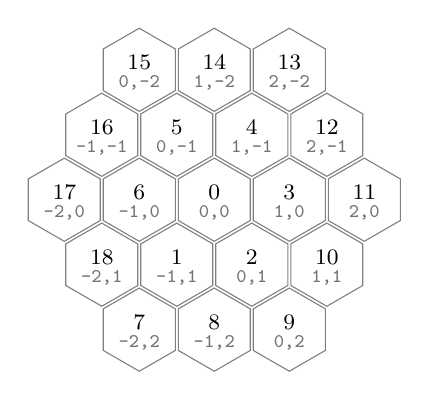
\begin{tikzpicture}\draw[black!50,line width=0.4pt] (0.457,-0.264) -- (0.457,0.264) -- (0.000,0.528) -- (-0.457,0.264) -- (-0.457,-0.264) -- (-0.000,-0.528) -- cycle;
\node[font=\footnotesize\sffamily] at (0.000,0.090) {0};
\node[font=\scriptsize\ttfamily,text=black!55] at (0.000,-0.170) {0,0};
\draw[black!50,line width=0.4pt] (-0.019,-1.089) -- (-0.019,-0.561) -- (-0.476,-0.297) -- (-0.934,-0.561) -- (-0.934,-1.089) -- (-0.476,-1.353) -- cycle;
\node[font=\footnotesize\sffamily] at (-0.476,-0.735) {1};
\node[font=\scriptsize\ttfamily,text=black!55] at (-0.476,-0.995) {-1,1};
\draw[black!50,line width=0.4pt] (0.934,-1.089) -- (0.934,-0.561) -- (0.476,-0.297) -- (0.019,-0.561) -- (0.019,-1.089) -- (0.476,-1.353) -- cycle;
\node[font=\footnotesize\sffamily] at (0.476,-0.735) {2};
\node[font=\scriptsize\ttfamily,text=black!55] at (0.476,-0.995) {0,1};
\draw[black!50,line width=0.4pt] (1.410,-0.264) -- (1.410,0.264) -- (0.953,0.528) -- (0.495,0.264) -- (0.495,-0.264) -- (0.953,-0.528) -- cycle;
\node[font=\footnotesize\sffamily] at (0.953,0.090) {3};
\node[font=\scriptsize\ttfamily,text=black!55] at (0.953,-0.170) {1,0};
\draw[black!50,line width=0.4pt] (0.934,0.561) -- (0.934,1.089) -- (0.476,1.353) -- (0.019,1.089) -- (0.019,0.561) -- (0.476,0.297) -- cycle;
\node[font=\footnotesize\sffamily] at (0.476,0.915) {4};
\node[font=\scriptsize\ttfamily,text=black!55] at (0.476,0.655) {1,-1};
\draw[black!50,line width=0.4pt] (-0.019,0.561) -- (-0.019,1.089) -- (-0.476,1.353) -- (-0.934,1.089) -- (-0.934,0.561) -- (-0.476,0.297) -- cycle;
\node[font=\footnotesize\sffamily] at (-0.476,0.915) {5};
\node[font=\scriptsize\ttfamily,text=black!55] at (-0.476,0.655) {0,-1};
\draw[black!50,line width=0.4pt] (-0.495,-0.264) -- (-0.495,0.264) -- (-0.953,0.528) -- (-1.410,0.264) -- (-1.410,-0.264) -- (-0.953,-0.528) -- cycle;
\node[font=\footnotesize\sffamily] at (-0.953,0.090) {6};
\node[font=\scriptsize\ttfamily,text=black!55] at (-0.953,-0.170) {-1,0};
\draw[black!50,line width=0.4pt] (-0.495,-1.914) -- (-0.495,-1.386) -- (-0.953,-1.122) -- (-1.410,-1.386) -- (-1.410,-1.914) -- (-0.953,-2.178) -- cycle;
\node[font=\footnotesize\sffamily] at (-0.953,-1.560) {7};
\node[font=\scriptsize\ttfamily,text=black!55] at (-0.953,-1.820) {-2,2};
\draw[black!50,line width=0.4pt] (0.457,-1.914) -- (0.457,-1.386) -- (0.000,-1.122) -- (-0.457,-1.386) -- (-0.457,-1.914) -- (-0.000,-2.178) -- cycle;
\node[font=\footnotesize\sffamily] at (0.000,-1.560) {8};
\node[font=\scriptsize\ttfamily,text=black!55] at (0.000,-1.820) {-1,2};
\draw[black!50,line width=0.4pt] (1.410,-1.914) -- (1.410,-1.386) -- (0.953,-1.122) -- (0.495,-1.386) -- (0.495,-1.914) -- (0.953,-2.178) -- cycle;
\node[font=\footnotesize\sffamily] at (0.953,-1.560) {9};
\node[font=\scriptsize\ttfamily,text=black!55] at (0.953,-1.820) {0,2};
\draw[black!50,line width=0.4pt] (1.886,-1.089) -- (1.886,-0.561) -- (1.429,-0.297) -- (0.972,-0.561) -- (0.972,-1.089) -- (1.429,-1.353) -- cycle;
\node[font=\footnotesize\sffamily] at (1.429,-0.735) {10};
\node[font=\scriptsize\ttfamily,text=black!55] at (1.429,-0.995) {1,1};
\draw[black!50,line width=0.4pt] (2.363,-0.264) -- (2.363,0.264) -- (1.905,0.528) -- (1.448,0.264) -- (1.448,-0.264) -- (1.905,-0.528) -- cycle;
\node[font=\footnotesize\sffamily] at (1.905,0.090) {11};
\node[font=\scriptsize\ttfamily,text=black!55] at (1.905,-0.170) {2,0};
\draw[black!50,line width=0.4pt] (1.886,0.561) -- (1.886,1.089) -- (1.429,1.353) -- (0.972,1.089) -- (0.972,0.561) -- (1.429,0.297) -- cycle;
\node[font=\footnotesize\sffamily] at (1.429,0.915) {12};
\node[font=\scriptsize\ttfamily,text=black!55] at (1.429,0.655) {2,-1};
\draw[black!50,line width=0.4pt] (1.410,1.386) -- (1.410,1.914) -- (0.953,2.178) -- (0.495,1.914) -- (0.495,1.386) -- (0.953,1.122) -- cycle;
\node[font=\footnotesize\sffamily] at (0.953,1.740) {13};
\node[font=\scriptsize\ttfamily,text=black!55] at (0.953,1.480) {2,-2};
\draw[black!50,line width=0.4pt] (0.457,1.386) -- (0.457,1.914) -- (0.000,2.178) -- (-0.457,1.914) -- (-0.457,1.386) -- (-0.000,1.122) -- cycle;
\node[font=\footnotesize\sffamily] at (0.000,1.740) {14};
\node[font=\scriptsize\ttfamily,text=black!55] at (0.000,1.480) {1,-2};
\draw[black!50,line width=0.4pt] (-0.495,1.386) -- (-0.495,1.914) -- (-0.953,2.178) -- (-1.410,1.914) -- (-1.410,1.386) -- (-0.953,1.122) -- cycle;
\node[font=\footnotesize\sffamily] at (-0.953,1.740) {15};
\node[font=\scriptsize\ttfamily,text=black!55] at (-0.953,1.480) {0,-2};
\draw[black!50,line width=0.4pt] (-0.972,0.561) -- (-0.972,1.089) -- (-1.429,1.353) -- (-1.886,1.089) -- (-1.886,0.561) -- (-1.429,0.297) -- cycle;
\node[font=\footnotesize\sffamily] at (-1.429,0.915) {16};
\node[font=\scriptsize\ttfamily,text=black!55] at (-1.429,0.655) {-1,-1};
\draw[black!50,line width=0.4pt] (-1.448,-0.264) -- (-1.448,0.264) -- (-1.905,0.528) -- (-2.363,0.264) -- (-2.363,-0.264) -- (-1.905,-0.528) -- cycle;
\node[font=\footnotesize\sffamily] at (-1.905,0.090) {17};
\node[font=\scriptsize\ttfamily,text=black!55] at (-1.905,-0.170) {-2,0};
\draw[black!50,line width=0.4pt] (-0.972,-1.089) -- (-0.972,-0.561) -- (-1.429,-0.297) -- (-1.886,-0.561) -- (-1.886,-1.089) -- (-1.429,-1.353) -- cycle;
\node[font=\footnotesize\sffamily] at (-1.429,-0.735) {18};
\node[font=\scriptsize\ttfamily,text=black!55] at (-1.429,-0.995) {-2,1};\end{tikzpicture}
\caption{Spiral indices on the board of radius 2. The small figures are the axial coordinates $(q,r)$.}
\label{fig:spiral}
\end{figure}

\begin{decision}{D1}{How large is the board, and what are empty cells?}
\textbf{Options.} (a) The host fixes a capacity $N$ at creation, the board is the smallest
$B_R$ with $|B_R|\ge N$, and unseated cells are void. (b) The board grows by a ring when it
fills. (c) The board has exactly as many cells as there are players, in an irregular shape.

\textbf{Recommendation: (a).} An image is planned against a fixed frame, and both (b) and (c)
move the frame during play. Void cells give the picture a background that no one controls,
and a host who wants a full board can set $N=|B_R|$. The default capacity is 61 ($R=4$).
Hosts may choose from 7 to 469 cells ($R\le 12$) in this version. That bound is set so that a
full board read stays a single explore deploy of modest cost, and can be raised once
\S\ref{sec:plan} Phase~4 has measured it.
\end{decision}

\subsection{Seating}\label{sec:seating}

A participant is seated by the \code{seat} move (\S\ref{sec:env}), which their client makes on
first entering an active or lobby instance. Seating is idempotent: a seated participant who calls
it again gets their existing cell.

\begin{decision}{D2}{Who chooses where a player sits?}
\textbf{Options.} (a) Random: the environment assigns a cell. (b) Claim: the player chooses a
free cell. (c) The host assigns cells.

\textbf{Recommendation: (a) by default, with (b) as a host option.} The deck's premise is that
a player's own actions are severely limited, and where you sit is an action with lasting
effect on who your neighbours are. Random seating keeps that choice out of the player's hands,
so neighbours who have never met must still negotiate. Claim seating suits games among
friends and tournaments with set formations. Host assignment adds a step every game would wait
on and is left out.

\textbf{Random seating, precisely.} Let $h=\mathrm{blake2b256}(\mathit{instance}\,\|\,\mathit{address})$
read as an unsigned integer. Starting at spiral index $h \bmod |B_R|$, the environment takes
the first free cell in increasing index order, wrapping at the end. The result depends only on
the instance, the address and the seats already taken, so anyone can check it. A player could
grind keys to steer the result. That is acceptable for a game and is noted in
\S\ref{sec:security}.
\end{decision}

\begin{decision}{D3}{What happens to a cell when its player leaves?}
\textbf{Options.} (a) The cell stays owned and keeps its last colour. (b) The cell becomes free
and void. (c) The cell becomes free and keeps its colour for the next occupant.

\textbf{Recommendation: (a).} A player who leaves through the Portal's \code{instances.leave}
keeps the seat. The client draws the cell dimmed, and rejoining restores control. Freeing cells
would let one player hold a sequence of cells by leaving and rejoining, and it would rewrite who
painted what in the history. A host who wants to recover seats closes the instance and starts
a new one.
\end{decision}

\subsection{Colour}

\begin{decision}{D4}{Which colours may a cell take?}
\textbf{Options.} (a) Any 24-bit sRGB colour. (b) A fixed palette. (c) Any colour by
default, with an optional palette set by the host.

\textbf{Recommendation: (c).} On the chain a colour is the string \code{\#RRGGBB} with
upper-case hexadecimal digits. The client offers a palette of 20 swatches, a free picker and
the player's recent colours. A host may restrict the instance to a palette of up to 32
colours. That is useful for themed games, for tournaments, and for boards meant to read as
pixel art. A cell that has never been painted is \emph{unpainted}, which is distinct from any
colour.
\end{decision}

\subsection{Phases}

F1R3Pix uses the Portal's instance status (\code{lobby}, \code{active}, \code{closed}), set only
by the host.

\begin{decision}{D5}{What may players do in each phase?}
\textbf{Recommendation.}

\begin{tabular}{@{}lccccc@{}}
\toprule
 & seat & paint & message & pay & read \\
\midrule
\code{lobby}  & yes & no  & yes & yes & yes\\
\code{active} & yes & yes & yes & yes & yes\\
\code{closed} & no  & no  & no  & no  & yes\\
\bottomrule
\end{tabular}

The lobby lets players gather, see the frame, sit down, talk and strike deals before anyone
paints, so a game can start together, as a tournament needs. Payment stays open in the lobby
because that is when deals are made. Closing freezes the board and the record.
\end{decision}

% ================================================================= 4
\section{Architecture}\label{sec:arch}

F1R3Pix adds no new kind of component to the Portal. It is one game environment on the shard,
one game client served from its own origin and framed by the Portal shell, and two additions
to the Portal (a \code{payments} domain in its environment and two host protocol methods).

\begin{figure}[ht]
\centering
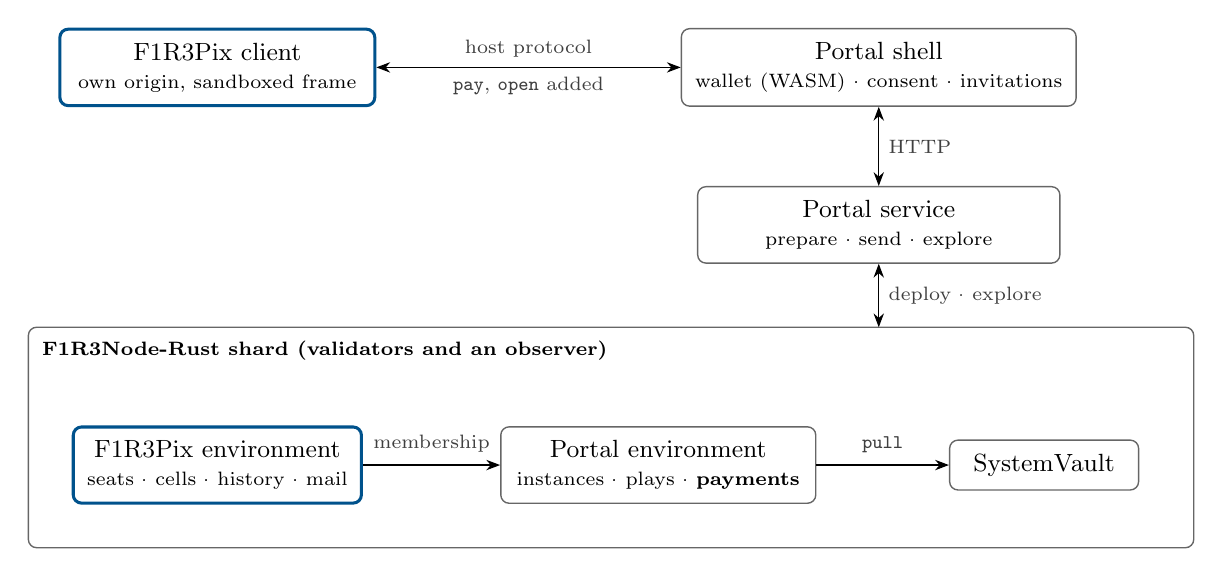
\begin{tikzpicture}[font=\small,
  box/.style={draw=black!60,line width=0.5pt,rounded corners=3pt,align=center,inner sep=5pt,fill=white},
  new/.style={box,draw=brandskydark,line width=1.1pt},
  lab/.style={font=\scriptsize,text=muted,align=center},
  >={Stealth[length=5pt]}]
  \node[new,minimum width=40mm] (game) at (0,0) {F1R3Pix client\\[-1pt]{\scriptsize own origin, sandboxed frame}};
  \node[box,minimum width=46mm] (shell) at (8.4,0) {Portal shell\\[-1pt]{\scriptsize wallet (WASM) · consent · invitations}};
  \node[box,minimum width=46mm] (svc) at (8.4,-2.0) {Portal service\\[-1pt]{\scriptsize prepare · send · explore}};
  \draw[black!60,rounded corners=3pt,line width=0.5pt] (-2.4,-3.3) rectangle (12.4,-6.1);
  \node[anchor=north west,font=\scriptsize\bfseries] at (-2.35,-3.35) {F1R3Node-Rust shard (validators and an observer)};
  \node[new,minimum width=36mm] (pixenv) at (0,-5.05) {F1R3Pix environment\\[-1pt]{\scriptsize seats · cells · history · mail}};
  \node[box,minimum width=40mm] (penv) at (5.6,-5.05) {Portal environment\\[-1pt]{\scriptsize instances · plays · \textbf{payments}}};
  \node[box,minimum width=24mm] (vault) at (10.5,-5.05) {SystemVault};
  \draw[<->] (game) -- node[above,lab]{host protocol}node[below,lab]{\code{pay}, \code{open} added} (shell);
  \draw[<->] (shell) -- node[right,lab]{HTTP} (svc);
  \draw[<->] (svc) -- node[right,lab]{deploy · explore} (8.4,-3.3);
  \draw[->] (pixenv) -- node[above,lab,yshift=1pt]{membership} (penv);
  \draw[->] (penv) -- node[above,lab,yshift=1pt]{\code{pull}} (vault);
\end{tikzpicture}
\caption{Components. Outlined in dark sky: what this design adds or replaces.}
\label{fig:arch}
\end{figure}

\subsection{Authority}

The design keeps the Portal's separation of authority intact.

\begin{itemize}[leftmargin=1.2em,itemsep=2pt]
\item The game client never sees a key. It reaches identity, the shard and payment only
  through the host protocol.
\item The F1R3Pix environment reads the caller's address, which it obtains from
  \code{rho:deploy:data} through \code{rho:vault:address}, and the block height (from \code{rho:block:data}), and nothing
  else. It never touches a vault.
\item Funds move only through the Portal environment's \code{payments.send}, signed only from
  the Portal shell and only after a prompt that names it as a payment.
\item Message plaintext is sealed in the game client and opened by the wallet. The chain holds
  only \mbox{ciphertext}.
\end{itemize}

% ================================================================= 5
\section{The F1R3Pix environment}\label{sec:env}

The environment replaces the installed \code{f1r3pix.rho} body inside the shared game
\code{prelude.rho}. It keeps the prelude's machinery: installation under the game's registry
key with \code{rho:registry:\allowbreak insertSigned:\allowbreak secp256k1}, version-checked upgrade, \code{who},
\code{member}, \code{instanceOf} and the \code{TreeHashMap} store. Installing it raises the
environment version, so the URI is unchanged and every call template's hash changes. The
manifest is then re-registered by the F1R3FLY.io Cooperative (\S\ref{sec:manifest}).

\subsection{Configuration}

The instance's configuration is the \code{config} map the host passes to the Portal's
\code{instances.create}. The environment reads it from the Portal's instance record instead of
keeping its own copy, so there is one source of truth. It is fixed at creation.

\begin{lstlisting}[language=rholang]
{ "capacity": 61,              // 7 ..= 469; the board is the smallest B_R that seats it
  "seating":  "random",        // "random" | "claim"                          (D2)
  "palette":  Nil,             // Nil, or a list of up to 32 "#RRGGBB"         (D4)
  "messageLimit": 2048 }       // bytes of sealed envelope per message      (sec. 6)
\end{lstlisting}

\req{r:config}~The environment \MUST{} refuse every move on an instance whose configuration is
missing or out of range, answering \code{(false, "bad config")}. It \MUSTNOT{} substitute defaults.
Defaults are applied by the client that creates the instance, where the host can see them.

\subsection{State}

All keys are scoped by instance, so instances never share state.

\begin{center}\small
\begin{tabularx}{\linewidth}{@{}>{\ttfamily}l X l@{}}
\toprule
\normalfont key & value & written by\\
\midrule
("seat", i, a)    & \code{\{"cell": [q, r], "pk": <public key>, "at": ts, "h": height\}} & \code{seat}, by $a$\\
("cell", i, q, r) & \code{\{"owner": a, "colour": c | Nil, "at": ts, "h": height, "n": count\}} & \code{seat}, \code{paint}\\
("hist", i, q, r) & list of \code{[h, ts, c]}, oldest first & \code{paint}\\
("out", i, a)     & list of envelopes, \S\ref{sec:mail} & \code{say}, by $a$\\
\bottomrule
\end{tabularx}
\end{center}

\req{r:single-writer}~After seating, every key \code{("cell", i, q, r)}, \code{("hist", i, q, r)}
and \code{("out", i, a)} has exactly one writer: the seated owner, or the sender. Two players
therefore never contend for the same key when they paint or send. \code{TreeHashMap} spreads
keys over a trie keyed by keccak-256 to depth 3, so distinct keys rarely share a leaf
either. This is the per-cell successor to the installed environment's per-row storage. It is
stronger, because ownership rules out two writers on the same key altogether.

The environment deliberately keeps no instance-wide counter or log, since every writer would
contend for it. Global order is recovered when reading (\S\ref{sec:order}).

\subsection{Moves}

Moves are play templates. Within the allowance granted at launch they are signed without a
prompt. Each answers \code{(true, value)} or \code{(false, reason)}.

\textbf{\code{seat(instance, pk, want)}.} Seats the caller. \code{pk} is the caller's
uncompressed secp256k1 public key, used to seal messages to them. \code{want} is \code{Nil}
under random seating, or \code{[q, r]} under claim seating.
\begin{itemize}[leftmargin=1.2em,itemsep=1pt]
\item Refuses unless the caller is a participant and the status is not \code{closed}.
\item Refuses unless \code{rho:vault:address}'s \code{"fromPublicKey"} applied to \code{pk}
  yields the caller's address, so no one can register a key that is not their own.
\item If the caller is already seated, answers their cell.
\item Under random seating, assigns the cell given by D2. Under claim seating, assigns
  \code{want} if it is on the board and free, and otherwise refuses with \code{"taken"}.
\item Refuses with \code{"full"} when every cell is seated.
\item Writes the seat and the cell's owner, unpainted. Answers \code{[q, r]}.
\end{itemize}

\textbf{\code{paint(instance, colour)}.} Sets the colour of the caller's own cell. The move
names no cell, because the only cell a player can paint is their own.
\begin{itemize}[leftmargin=1.2em,itemsep=1pt]
\item Refuses unless the caller is a participant, the status is \code{active}, and the caller
  is seated.
\item Refuses unless \code{colour} is seven characters: \code{\#} followed by six of
  \code{0123456789ABCDEF}. If the instance has a palette, also refuses unless \code{colour} is
  in it.
\item Reads the block height $h$ and the deploy timestamp $ts$. Writes the cell with
  \code{n} incremented, and appends \code{[h, ts, colour]} to the cell's history.
\item Answers \code{\{"cell": [q, r], "colour": colour, "h": h\}}.
\end{itemize}

\textbf{\code{say(instance, to, envelope)}.} Appends a sealed message to the caller's outbox.
\begin{itemize}[leftmargin=1.2em,itemsep=1pt]
\item Refuses unless the caller is a participant and the status is not \code{closed}.
\item Refuses unless \code{to} is a non-empty list of at most 64 distinct seated participants,
  none of them the caller.
\item Refuses unless \code{envelope} is a byte array no longer than the configured
  \code{messageLimit}.
\item Appends \code{\{"seq": n, "to": to, "env": envelope, "at": ts, "h": h\}}, where $n$ is
  the outbox's length before the append. Answers $n$.
\end{itemize}

\subsection{Reads}

Reads are explore deploys served by the observer. They cost the reader nothing and need no
signature.

\begin{center}\small
\begin{tabularx}{\linewidth}{@{}>{\ttfamily}l X@{}}
\toprule
\normalfont template & answers\\
\midrule
f1r3pix.board(instance)     & \code{\{"radius", "capacity", "palette", "status", "cells": [...]\}}: every seated cell with owner, colour, \code{at}, \code{h} and \code{n}; void cells are absent\\
f1r3pix.seats(instance)     & map from address to \code{\{"cell", "pk"\}}, for highlighting and for sealing\\
f1r3pix.log(instance, from, to) & every paint with $\mathit{from}\le h<\mathit{to}$, as \code{[h, ts, owner, q, r, colour]}, in the order of \S\ref{sec:order}\\
f1r3pix.mail(instance, address, cursor) & every envelope addressed to \code{address} after \code{cursor}, a map from sender to the last \code{seq} seen\\
f1r3pix.outbox(instance, address, from) & the address's own sent envelopes from \code{seq} onwards\\
\bottomrule
\end{tabularx}
\end{center}

Every read result also carries the block hash it reflects, as the Portal's reads do.

\subsection{Order and time}\label{sec:order}

A paint is stamped with the height of the block that includes it and the deploy timestamp the
painter signed. History is ordered by height, then timestamp, then owner address, then
the order of paints within a cell. Height is authoritative: the shard sets it. The timestamp
orders paints within a block. It is chosen by the deployer, within the node's acceptance
window, so a player can nudge their own paint's position within a block but not move it to
another block. For an outcome measured in frames that is immaterial, and the playback
renderer (\S\ref{sec:gallery}) groups by block.

\subsection{Contention}

Seating is the only move where two players can write the same key: two concurrent random seats
can hash to the same free cell, and two claims can name it. The environment reads and writes
the cell in one step, so concurrent seats of one cell conflict on that key and are settled by
the shard's ordinary conflict handling. The client \MUST{} treat a seat that was not included,
or that answers \code{"taken"}, as retryable.

\subsection{A sketch of \code{paint}}

\begin{lstlisting}[language=rholang]
contract env(@"paint", @instance, @colour, ret) = {
  new whoCh, rCh, sCh, hCh, ack1, ack2 in {
    who!(*whoCh) |
    for (@by, @ts <- whoCh) {
      // participant? status "active"? config valid? colour valid?
      ready!(instance, by, "active", colour, *rCh) |
      for (@ok, @why <- rCh) {
        if (not ok) { ret!((false, why)) }
        else {
          TreeHashMap!("get", state, ("seat", instance, by), *sCh) |
          for (@seat <- sCh) {
            match seat {
              Nil => { ret!((false, "take a seat first")) }
              _ => { match seat.get("cell") { [q, r] => {
                height!(*hCh) |
                for (@h <- hCh) {
                  update!(("cell", instance, q, r), colour, ts, h, *ack1) |
                  append!(("hist", instance, q, r), [h, ts, colour], *ack2) |
                  for (_ <- ack1 & _ <- ack2) {
                    ret!((true, {"cell": [q, r], "colour": colour, "h": h}))
                  }
                }
              } } }
            }
          }
        }
      }
    }
  }
}
\end{lstlisting}

\code{ready}, \code{height}, \code{update} and \code{append} are prelude-level helpers; \code{ready}
performs the participant, status, configuration and colour checks listed above. \code{height} is the Portal environment's existing helper over \code{rho:block:data}.

% ================================================================= 6
\section{Messages}\label{sec:mail}

\subsection{Where messages live}

\begin{decision}{D6}{On the chain or off it, and in the clear or sealed?}
\textbf{Options.} (a) On the chain in plain text. (b) On the chain, sealed to the recipients.
(c) Relayed off the chain by the Portal service, with only a hash on the chain.

\textbf{Recommendation: (b).} The suite's premise is that \emph{using F1R3FLY} any player can
communicate with any other, so messages belong on the shard, with the same durability and
ordering as moves. Plain text (a) would publish every negotiation permanently to anyone who
reads the shard. A relay (c) is faster and cheaper, but it puts a server the players must
trust between them, and it is not a F1R3FLY channel. Under (b) the sender, the recipient list,
the time and the size are public. The content is readable only by the recipients and the
sender.
\end{decision}

Each message is a deploy, so it costs phlo and arrives with the next block. That is a
deliberate trait of the game: talk is cheap but not free, and it moves at the shard's pace.
Message moves are play templates and are signed within the allowance without a prompt.
The default limit is 2,048 bytes of envelope per message. That leaves about 1,800 bytes of
text for one recipient, since the fixed part of the envelope takes about 110 bytes and each
recipient, the sender included, adds a wrap of about 85.

\subsection{Sealing}\label{sec:sealing}

The envelope uses only primitives the Portal wallet already carries (\code{k256},
\code{hkdf} with SHA-256, \code{aes-gcm}), so sealing adds no dependency.

\begin{enumerate}[leftmargin=1.4em,itemsep=2pt]
\item The client draws a random 32-byte content key $K$ and an ephemeral secp256k1 key pair
  $(e,E)$.
\item The body is
  \[C=\mathrm{AES\text{-}256\text{-}GCM}_K(\mathit{nonce}_0,\ \mathit{plaintext},\ \mathit{aad}),\qquad
    \mathit{aad} = \text{\code{"f1r3pix/msg/v1"}}\,\|\,\mathit{instance}\,\|\,\mathit{sender}.\]
\item For each recipient $j$, and for the sender (so the sender can reread their own sent
  messages), the client computes $Z_j=\mathrm{ECDH}(e, P_j)$ with $P_j$ from
  \code{f1r3pix.seats}, derives
  \[W_j=\mathrm{HKDF}(Z_j,\ \mathit{salt}=E,\ \mathit{info}=\text{\code{"f1r3pix/msg/v1"}}\,\|\,\mathit{instance}),\]
  and wraps $K$ as $\mathrm{AES\text{-}256\text{-}GCM}_{W_j}(\mathit{nonce}_j, K)$.
\item The envelope is the CBOR map \code{\{v: 1, E, nonce$_0$, C, wraps: [[address, nonce, wrapped K], ...]\}}.
\end{enumerate}

Sealing needs only public keys, so the game client does it itself. Opening needs the
recipient's private key, so it is done by the wallet through the host protocol's new
\code{open} method (\S\ref{sec:host}).

\req{r:open-scope}~The host \MUST{} pass the wallet the game id and instance of the frame it is
hosting, and the wallet \MUST{} use them in \code{info} and \code{aad}. A game frame then cannot
use \code{open} to read envelopes made for another game or another instance. That holds even
for the user's own envelopes.

The identity key is a signing key, and \code{open} also uses it for ECDH. This is the usual
ECIES practice, and the \code{info} string keeps the derived keys separate from every other use.
If F1R3FLY later adopts a separate key for encryption, the envelope version changes and
\code{seats} carries that key instead.

\subsection{What sealing does not protect}

The game client sees the plaintext, because the player types it there. Sealing protects
messages from readers of the chain, not from the game client. That is the same trust a player
already places in a game they choose to load. Recipient lists are public, so the shape of the
negotiation (who talks to whom, how often) is visible to everyone. A player who needs that
hidden can use other channels. Hiding recipients is left for a later version
(\S\ref{sec:future}).

% ================================================================= 7
\section{Payments}\label{sec:pay}

\subsection{The payments domain}

Paying is one of the game's three actions, and the Portal has no way for a game to do it
(Findings 2 and 4, \S\ref{sec:findings}). F1R3Pix needs a payment path that:

\begin{itemize}[leftmargin=1.2em,itemsep=1pt]
\item never lets a game sign anything that moves funds;
\item lets a game ask for a payment to players it has selected;
\item keeps a record of payments within an instance that can be trusted as much as the chain;
\item will also serve tournament antes later, and any other game that pays.
\end{itemize}

It belongs in the Portal environment, which already moves funds for sponsorships through its
\code{pull} helper, and not in the game environment. It follows the Embers pattern: the
contract that moves the funds also keeps the history, so the history is as authoritative as
the transfers.

\textbf{\code{payments.send(instanceId, transfers, memo)}.} \code{transfers} is a list of
\code{[to, amount]}.
\begin{itemize}[leftmargin=1.2em,itemsep=1pt]
\item Refuses unless the caller is a participant of the instance and its status is not
  \code{closed}.
\item Refuses unless there are between 1 and 64 transfers, every \code{to} is a distinct
  participant other than the caller, and every amount is a positive integer.
\item Refuses unless \code{memo} is \code{Nil} or a string of at most 140 characters. The memo
  is public.
\item For each transfer in order, calls \code{pull} from the caller's vault and records
  \code{\{"seq", "to", "amount", "ok", "reason", "at", "h", "memo"\}} under
  \code{("pay", instanceId, caller)}, which only the caller writes.
\item Answers the list of per-transfer results.
\end{itemize}
Transfers are independent. If the vault refuses one (for instance, because the balance ran
out), the ones before it stand, and the record says which. The client checks the balance and
shows the total before asking, so this case is rare.

\textbf{\code{payments.list(instanceId, cursor)}.} An explore read. It answers every payment
within the instance after \code{cursor}, merged by height, from the records of each
participant.

\req{r:moves-funds}~\code{payments.send} \MUST{} be added to the catalogue's
\code{MOVES\_FUNDS}. The wallet \MUST{} sign it only from the Portal origin, always after a
prompt, and \MUSTNOT{} sign it within an allowance.

\subsection{The amount}

\begin{decision}{D7}{When several players are selected, what does the amount mean?}
\textbf{Options.} (a) Each: the amount is sent to every selected player. (b) Split: the amount
is divided among them. (c) Both, chosen by the player.

\textbf{Recommendation: (c), with \emph{each} as the default.} Most deals in the game are of the
form ``five each if you all turn blue'', which is \emph{each}. \emph{Split} suits paying a block
for a shared result. The send control shows a toggle and, before anything is signed, the line
\emph{``10 each to 3 players: 30 F1R3Cap''} or \emph{``30 split among 3 players: 10 each''}. A
split that does not divide evenly in the vault's base unit is refused, and the control
suggests the nearest amount that does. The prototype's silent loss of the remainder is
removed.
\end{decision}

\subsection{The flow}

\begin{figure}[h]
\centering
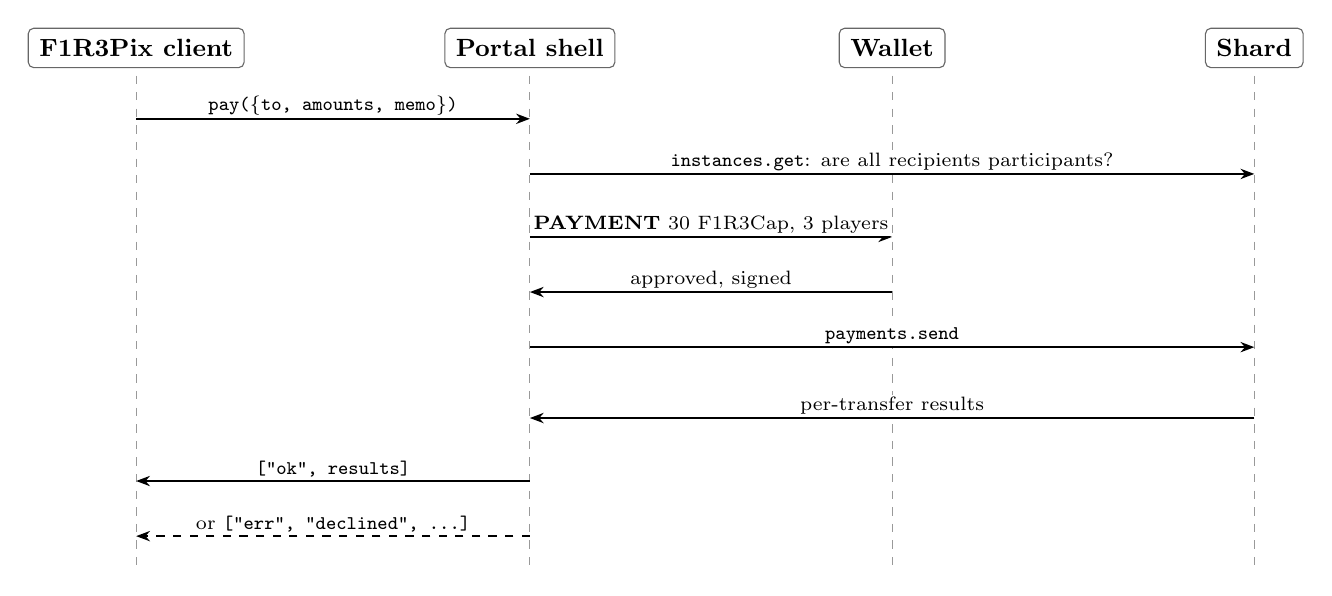
\begin{tikzpicture}[font=\small,>={Stealth[length=5pt]},
  life/.style={draw=black!40,dashed},
  hd/.style={draw=black!60,rounded corners=2pt,fill=white,inner sep=4pt,font=\small\bfseries},
  msg/.style={->,line width=0.5pt},
  lab/.style={font=\scriptsize,fill=white,inner sep=1pt}]
  \foreach \x/\n/\t in {0/g/F1R3Pix client,5/s/Portal shell,9.6/w/Wallet,14.2/c/Shard}{
    \node[hd] (\n) at (\x,0) {\t};
    \draw[life] (\x,-0.35) -- (\x,-6.6);
  }
  \draw[msg] (0,-0.9) -- node[lab,above]{\code{pay(\{to, amounts, memo\})}} (5,-0.9);
  \draw[msg] (5,-1.6) -- node[lab,above]{\code{instances.get}: are all recipients participants?} (14.2,-1.6);
  \draw[msg] (5,-2.4) -- node[lab,above]{\textbf{PAYMENT} 30 F1R3Cap, 3 players} (9.6,-2.4);
  \draw[msg] (9.6,-3.1) -- node[lab,above]{approved, signed} (5,-3.1);
  \draw[msg] (5,-3.8) -- node[lab,above]{\code{payments.send}} (14.2,-3.8);
  \draw[msg] (14.2,-4.7) -- node[lab,above]{per-transfer results} (5,-4.7);
  \draw[msg] (5,-5.5) -- node[lab,above]{\code{["ok", results]}} (0,-5.5);
  \draw[msg,dashed] (5,-6.2) -- node[lab,above]{or \code{["err", "declined", ...]}} (0,-6.2);
\end{tikzpicture}
\caption{A payment. The game asks; the shell checks the recipients, the person approves, the shell signs and sends.}
\label{fig:payflow}
\end{figure}

\req{r:pay-check}~The shell \MUST{} refuse a \code{pay} request naming anyone who is not a
participant of the hosted instance, before showing a prompt. The environment makes the same check
on the chain. The shell's check exists so that a misbehaving game frame cannot even put a
prompt for an outside address in front of the player.

% ================================================================= 8
\section{Host protocol additions}\label{sec:host}

Two methods are added to \code{core/host.ts} and to the game SDK. Both follow the protocol's
existing conventions: \code{["ok", value]} or \code{["err", code, message]}.

\begin{center}\small
\begin{tabularx}{\linewidth}{@{}>{\ttfamily}l X@{}}
\toprule
\normalfont method & behaviour\\
\midrule
pay(\{to, amounts, memo\}) & Checks that every recipient is a participant of the hosted instance (R\ref{r:pay-check}), shows the payment prompt, signs \code{payments.send} on approval and sends it. Errors: \code{not-participant}, \code{declined}, \code{insufficient}, \code{node}.\\
open(\{envelope\}) & Asks the wallet to open an envelope addressed to the active address, with the hosted game id and instance bound into the derivation (R\ref{r:open-scope}). Answers the plaintext. Errors: \code{not-addressed}, \code{corrupt}. Never prompts.\\
\bottomrule
\end{tabularx}
\end{center}

\code{open} never prompts because it reveals nothing the player could not already read, and it
reveals it only to the game frame they are playing. The wallet \MUST{} still rate-limit it, at a
default of 50 calls per second, so a broken game cannot pin the WASM thread.

Neither method is specific to F1R3Pix. Any game whose manifest declares the capability may use
them. The manifest gains a \code{"capabilities": ["pay", "open"]} list. The host refuses
methods a game has not declared, and the Portal shows a game's capabilities on its card before
launch.

% ================================================================= 9
\section{The client}\label{sec:client}

The client is a web page served from the game's own origin and framed by the Portal. To serve
the same purpose as the Portal shell, as a test bed for doing this in F1R3Gaze, it follows the
shell's structure: a framework-free TypeScript core holding every operation, and a React layer
that only renders. In F1R3Gaze each core operation becomes a f1r3lang process over the
attenuated \code{portal} capability (\S\ref{sec:gaze}).

\subsection{Layout}

The page has three columns. The centre column is the widest and holds the board, because the
board is where attention belongs.

\begin{figure}[h]
\centering
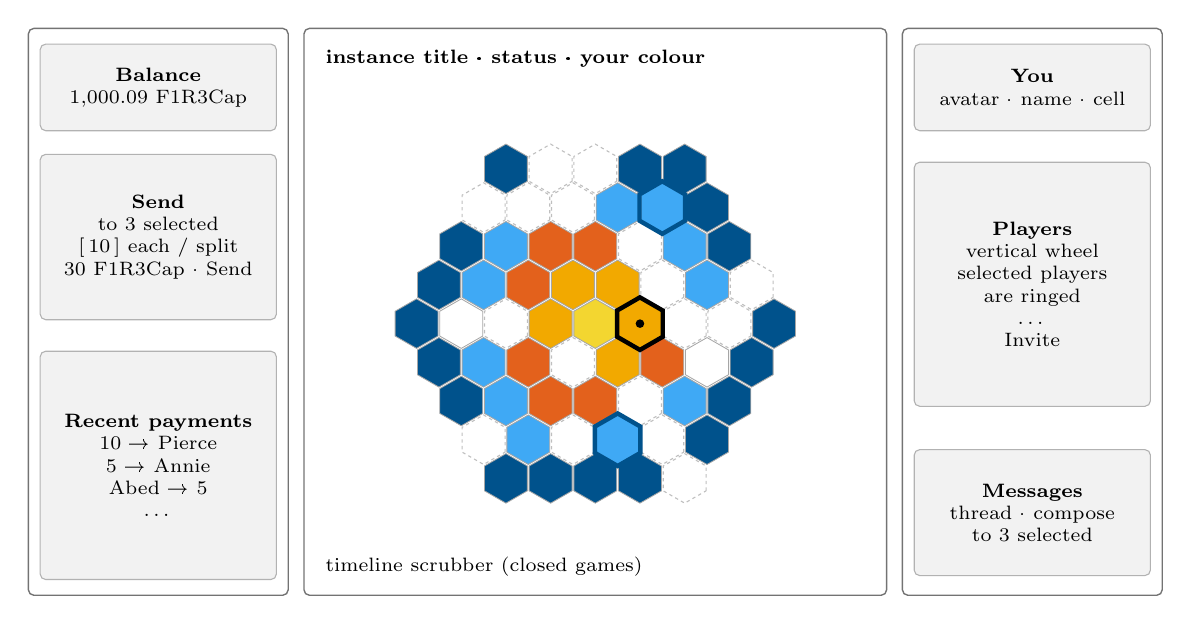
\begin{tikzpicture}[font=\scriptsize,
  col/.style={draw=black!55,line width=0.5pt,rounded corners=2pt},
  pane/.style={draw=black!30,rounded corners=2pt,fill=codebg,align=center,inner sep=2pt}]
  \draw[col] (0,0) rectangle (3.3,7.2);
  \draw[col] (3.5,0) rectangle (10.9,7.2);
  \draw[col] (11.1,0) rectangle (14.4,7.2);
  % left
  \node[pane,minimum width=30mm,minimum height=11mm] at (1.65,6.45) {\textbf{Balance}\\1,000.09 F1R3Cap};
  \node[pane,minimum width=30mm,minimum height=21mm] at (1.65,4.55) {\textbf{Send}\\to 3 selected\\{[}\,10\,{]} each / split\\30 F1R3Cap · Send};
  \node[pane,minimum width=30mm,minimum height=29mm] at (1.65,1.65) {\textbf{Recent payments}\\10 \textrightarrow{} Pierce\\5 \textrightarrow{} Annie\\Abed \textrightarrow{} 5\\\ldots};
  % centre
  \node[anchor=north west,font=\scriptsize\bfseries] at (3.65,7.05) {instance title · status · your colour};
  \begin{scope}[shift={(7.2,3.45)},scale=0.78]\fill[fill={rgb,255:red,243;green,214;blue,48}] (0.349,-0.202) -- (0.349,0.202) -- (0.000,0.403) -- (-0.349,0.202) -- (-0.349,-0.202) -- (-0.000,-0.403) -- cycle;
\draw[black!35,line width=0.3pt] (0.349,-0.202) -- (0.349,0.202) -- (0.000,0.403) -- (-0.349,0.202) -- (-0.349,-0.202) -- (-0.000,-0.403) -- cycle;
\draw[black!25,line width=0.4pt,dash pattern=on 1.2pt off 1.2pt] (-0.015,-0.832) -- (-0.015,-0.428) -- (-0.364,-0.227) -- (-0.713,-0.428) -- (-0.713,-0.832) -- (-0.364,-1.033) -- cycle;
\fill[fill={rgb,255:red,242;green,169;blue,0}] (0.713,-0.832) -- (0.713,-0.428) -- (0.364,-0.227) -- (0.015,-0.428) -- (0.015,-0.832) -- (0.364,-1.033) -- cycle;
\draw[black!35,line width=0.3pt] (0.713,-0.832) -- (0.713,-0.428) -- (0.364,-0.227) -- (0.015,-0.428) -- (0.015,-0.832) -- (0.364,-1.033) -- cycle;
\fill[fill={rgb,255:red,242;green,169;blue,0}] (1.077,-0.202) -- (1.077,0.202) -- (0.727,0.403) -- (0.378,0.202) -- (0.378,-0.202) -- (0.727,-0.403) -- cycle;
\draw[black!35,line width=0.3pt] (1.077,-0.202) -- (1.077,0.202) -- (0.727,0.403) -- (0.378,0.202) -- (0.378,-0.202) -- (0.727,-0.403) -- cycle;
\fill[fill={rgb,255:red,242;green,169;blue,0}] (0.713,0.428) -- (0.713,0.832) -- (0.364,1.033) -- (0.015,0.832) -- (0.015,0.428) -- (0.364,0.227) -- cycle;
\draw[black!35,line width=0.3pt] (0.713,0.428) -- (0.713,0.832) -- (0.364,1.033) -- (0.015,0.832) -- (0.015,0.428) -- (0.364,0.227) -- cycle;
\fill[fill={rgb,255:red,242;green,169;blue,0}] (-0.015,0.428) -- (-0.015,0.832) -- (-0.364,1.033) -- (-0.713,0.832) -- (-0.713,0.428) -- (-0.364,0.227) -- cycle;
\draw[black!35,line width=0.3pt] (-0.015,0.428) -- (-0.015,0.832) -- (-0.364,1.033) -- (-0.713,0.832) -- (-0.713,0.428) -- (-0.364,0.227) -- cycle;
\fill[fill={rgb,255:red,242;green,169;blue,0}] (-0.378,-0.202) -- (-0.378,0.202) -- (-0.727,0.403) -- (-1.077,0.202) -- (-1.077,-0.202) -- (-0.727,-0.403) -- cycle;
\draw[black!35,line width=0.3pt] (-0.378,-0.202) -- (-0.378,0.202) -- (-0.727,0.403) -- (-1.077,0.202) -- (-1.077,-0.202) -- (-0.727,-0.403) -- cycle;
\fill[fill={rgb,255:red,227;green,97;blue,28}] (-0.378,-1.462) -- (-0.378,-1.058) -- (-0.727,-0.857) -- (-1.077,-1.058) -- (-1.077,-1.462) -- (-0.727,-1.663) -- cycle;
\draw[black!35,line width=0.3pt] (-0.378,-1.462) -- (-0.378,-1.058) -- (-0.727,-0.857) -- (-1.077,-1.058) -- (-1.077,-1.462) -- (-0.727,-1.663) -- cycle;
\fill[fill={rgb,255:red,227;green,97;blue,28}] (0.349,-1.462) -- (0.349,-1.058) -- (0.000,-0.857) -- (-0.349,-1.058) -- (-0.349,-1.462) -- (-0.000,-1.663) -- cycle;
\draw[black!35,line width=0.3pt] (0.349,-1.462) -- (0.349,-1.058) -- (0.000,-0.857) -- (-0.349,-1.058) -- (-0.349,-1.462) -- (-0.000,-1.663) -- cycle;
\draw[black!25,line width=0.4pt,dash pattern=on 1.2pt off 1.2pt] (1.077,-1.462) -- (1.077,-1.058) -- (0.727,-0.857) -- (0.378,-1.058) -- (0.378,-1.462) -- (0.727,-1.663) -- cycle;
\fill[fill={rgb,255:red,227;green,97;blue,28}] (1.440,-0.832) -- (1.440,-0.428) -- (1.091,-0.227) -- (0.742,-0.428) -- (0.742,-0.832) -- (1.091,-1.033) -- cycle;
\draw[black!35,line width=0.3pt] (1.440,-0.832) -- (1.440,-0.428) -- (1.091,-0.227) -- (0.742,-0.428) -- (0.742,-0.832) -- (1.091,-1.033) -- cycle;
\draw[black!25,line width=0.4pt,dash pattern=on 1.2pt off 1.2pt] (1.804,-0.202) -- (1.804,0.202) -- (1.455,0.403) -- (1.106,0.202) -- (1.106,-0.202) -- (1.455,-0.403) -- cycle;
\draw[black!25,line width=0.4pt,dash pattern=on 1.2pt off 1.2pt] (1.440,0.428) -- (1.440,0.832) -- (1.091,1.033) -- (0.742,0.832) -- (0.742,0.428) -- (1.091,0.227) -- cycle;
\draw[black!25,line width=0.4pt,dash pattern=on 1.2pt off 1.2pt] (1.077,1.058) -- (1.077,1.462) -- (0.727,1.663) -- (0.378,1.462) -- (0.378,1.058) -- (0.727,0.857) -- cycle;
\fill[fill={rgb,255:red,227;green,97;blue,28}] (0.349,1.058) -- (0.349,1.462) -- (0.000,1.663) -- (-0.349,1.462) -- (-0.349,1.058) -- (-0.000,0.857) -- cycle;
\draw[black!35,line width=0.3pt] (0.349,1.058) -- (0.349,1.462) -- (0.000,1.663) -- (-0.349,1.462) -- (-0.349,1.058) -- (-0.000,0.857) -- cycle;
\fill[fill={rgb,255:red,227;green,97;blue,28}] (-0.378,1.058) -- (-0.378,1.462) -- (-0.727,1.663) -- (-1.077,1.462) -- (-1.077,1.058) -- (-0.727,0.857) -- cycle;
\draw[black!35,line width=0.3pt] (-0.378,1.058) -- (-0.378,1.462) -- (-0.727,1.663) -- (-1.077,1.462) -- (-1.077,1.058) -- (-0.727,0.857) -- cycle;
\fill[fill={rgb,255:red,227;green,97;blue,28}] (-0.742,0.428) -- (-0.742,0.832) -- (-1.091,1.033) -- (-1.440,0.832) -- (-1.440,0.428) -- (-1.091,0.227) -- cycle;
\draw[black!35,line width=0.3pt] (-0.742,0.428) -- (-0.742,0.832) -- (-1.091,1.033) -- (-1.440,0.832) -- (-1.440,0.428) -- (-1.091,0.227) -- cycle;
\draw[black!25,line width=0.4pt,dash pattern=on 1.2pt off 1.2pt] (-1.106,-0.202) -- (-1.106,0.202) -- (-1.455,0.403) -- (-1.804,0.202) -- (-1.804,-0.202) -- (-1.455,-0.403) -- cycle;
\fill[fill={rgb,255:red,227;green,97;blue,28}] (-0.742,-0.832) -- (-0.742,-0.428) -- (-1.091,-0.227) -- (-1.440,-0.428) -- (-1.440,-0.832) -- (-1.091,-1.033) -- cycle;
\draw[black!35,line width=0.3pt] (-0.742,-0.832) -- (-0.742,-0.428) -- (-1.091,-0.227) -- (-1.440,-0.428) -- (-1.440,-0.832) -- (-1.091,-1.033) -- cycle;
\fill[fill={rgb,255:red,63;green,169;blue,245}] (-0.742,-2.092) -- (-0.742,-1.688) -- (-1.091,-1.487) -- (-1.440,-1.688) -- (-1.440,-2.092) -- (-1.091,-2.293) -- cycle;
\draw[black!35,line width=0.3pt] (-0.742,-2.092) -- (-0.742,-1.688) -- (-1.091,-1.487) -- (-1.440,-1.688) -- (-1.440,-2.092) -- (-1.091,-2.293) -- cycle;
\draw[black!25,line width=0.4pt,dash pattern=on 1.2pt off 1.2pt] (-0.015,-2.092) -- (-0.015,-1.688) -- (-0.364,-1.487) -- (-0.713,-1.688) -- (-0.713,-2.092) -- (-0.364,-2.293) -- cycle;
\fill[fill={rgb,255:red,63;green,169;blue,245}] (0.713,-2.092) -- (0.713,-1.688) -- (0.364,-1.487) -- (0.015,-1.688) -- (0.015,-2.092) -- (0.364,-2.293) -- cycle;
\draw[black!35,line width=0.3pt] (0.713,-2.092) -- (0.713,-1.688) -- (0.364,-1.487) -- (0.015,-1.688) -- (0.015,-2.092) -- (0.364,-2.293) -- cycle;
\draw[black!25,line width=0.4pt,dash pattern=on 1.2pt off 1.2pt] (1.440,-2.092) -- (1.440,-1.688) -- (1.091,-1.487) -- (0.742,-1.688) -- (0.742,-2.092) -- (1.091,-2.293) -- cycle;
\fill[fill={rgb,255:red,63;green,169;blue,245}] (1.804,-1.462) -- (1.804,-1.058) -- (1.455,-0.857) -- (1.106,-1.058) -- (1.106,-1.462) -- (1.455,-1.663) -- cycle;
\draw[black!35,line width=0.3pt] (1.804,-1.462) -- (1.804,-1.058) -- (1.455,-0.857) -- (1.106,-1.058) -- (1.106,-1.462) -- (1.455,-1.663) -- cycle;
\fill[fill={rgb,255:red,255;green,255;blue,255}] (2.168,-0.832) -- (2.168,-0.428) -- (1.819,-0.227) -- (1.469,-0.428) -- (1.469,-0.832) -- (1.819,-1.033) -- cycle;
\draw[black!35,line width=0.3pt] (2.168,-0.832) -- (2.168,-0.428) -- (1.819,-0.227) -- (1.469,-0.428) -- (1.469,-0.832) -- (1.819,-1.033) -- cycle;
\draw[black!25,line width=0.4pt,dash pattern=on 1.2pt off 1.2pt] (2.532,-0.202) -- (2.532,0.202) -- (2.182,0.403) -- (1.833,0.202) -- (1.833,-0.202) -- (2.182,-0.403) -- cycle;
\fill[fill={rgb,255:red,63;green,169;blue,245}] (2.168,0.428) -- (2.168,0.832) -- (1.819,1.033) -- (1.469,0.832) -- (1.469,0.428) -- (1.819,0.227) -- cycle;
\draw[black!35,line width=0.3pt] (2.168,0.428) -- (2.168,0.832) -- (1.819,1.033) -- (1.469,0.832) -- (1.469,0.428) -- (1.819,0.227) -- cycle;
\fill[fill={rgb,255:red,63;green,169;blue,245}] (1.804,1.058) -- (1.804,1.462) -- (1.455,1.663) -- (1.106,1.462) -- (1.106,1.058) -- (1.455,0.857) -- cycle;
\draw[black!35,line width=0.3pt] (1.804,1.058) -- (1.804,1.462) -- (1.455,1.663) -- (1.106,1.462) -- (1.106,1.058) -- (1.455,0.857) -- cycle;
\fill[fill={rgb,255:red,63;green,169;blue,245}] (1.440,1.688) -- (1.440,2.092) -- (1.091,2.293) -- (0.742,2.092) -- (0.742,1.688) -- (1.091,1.487) -- cycle;
\draw[black!35,line width=0.3pt] (1.440,1.688) -- (1.440,2.092) -- (1.091,2.293) -- (0.742,2.092) -- (0.742,1.688) -- (1.091,1.487) -- cycle;
\fill[fill={rgb,255:red,63;green,169;blue,245}] (0.713,1.688) -- (0.713,2.092) -- (0.364,2.293) -- (0.015,2.092) -- (0.015,1.688) -- (0.364,1.487) -- cycle;
\draw[black!35,line width=0.3pt] (0.713,1.688) -- (0.713,2.092) -- (0.364,2.293) -- (0.015,2.092) -- (0.015,1.688) -- (0.364,1.487) -- cycle;
\draw[black!25,line width=0.4pt,dash pattern=on 1.2pt off 1.2pt] (-0.015,1.688) -- (-0.015,2.092) -- (-0.364,2.293) -- (-0.713,2.092) -- (-0.713,1.688) -- (-0.364,1.487) -- cycle;
\draw[black!25,line width=0.4pt,dash pattern=on 1.2pt off 1.2pt] (-0.742,1.688) -- (-0.742,2.092) -- (-1.091,2.293) -- (-1.440,2.092) -- (-1.440,1.688) -- (-1.091,1.487) -- cycle;
\fill[fill={rgb,255:red,63;green,169;blue,245}] (-1.106,1.058) -- (-1.106,1.462) -- (-1.455,1.663) -- (-1.804,1.462) -- (-1.804,1.058) -- (-1.455,0.857) -- cycle;
\draw[black!35,line width=0.3pt] (-1.106,1.058) -- (-1.106,1.462) -- (-1.455,1.663) -- (-1.804,1.462) -- (-1.804,1.058) -- (-1.455,0.857) -- cycle;
\fill[fill={rgb,255:red,63;green,169;blue,245}] (-1.469,0.428) -- (-1.469,0.832) -- (-1.819,1.033) -- (-2.168,0.832) -- (-2.168,0.428) -- (-1.819,0.227) -- cycle;
\draw[black!35,line width=0.3pt] (-1.469,0.428) -- (-1.469,0.832) -- (-1.819,1.033) -- (-2.168,0.832) -- (-2.168,0.428) -- (-1.819,0.227) -- cycle;
\fill[fill={rgb,255:red,255;green,255;blue,255}] (-1.833,-0.202) -- (-1.833,0.202) -- (-2.182,0.403) -- (-2.532,0.202) -- (-2.532,-0.202) -- (-2.182,-0.403) -- cycle;
\draw[black!35,line width=0.3pt] (-1.833,-0.202) -- (-1.833,0.202) -- (-2.182,0.403) -- (-2.532,0.202) -- (-2.532,-0.202) -- (-2.182,-0.403) -- cycle;
\fill[fill={rgb,255:red,63;green,169;blue,245}] (-1.469,-0.832) -- (-1.469,-0.428) -- (-1.819,-0.227) -- (-2.168,-0.428) -- (-2.168,-0.832) -- (-1.819,-1.033) -- cycle;
\draw[black!35,line width=0.3pt] (-1.469,-0.832) -- (-1.469,-0.428) -- (-1.819,-0.227) -- (-2.168,-0.428) -- (-2.168,-0.832) -- (-1.819,-1.033) -- cycle;
\fill[fill={rgb,255:red,63;green,169;blue,245}] (-1.106,-1.462) -- (-1.106,-1.058) -- (-1.455,-0.857) -- (-1.804,-1.058) -- (-1.804,-1.462) -- (-1.455,-1.663) -- cycle;
\draw[black!35,line width=0.3pt] (-1.106,-1.462) -- (-1.106,-1.058) -- (-1.455,-0.857) -- (-1.804,-1.058) -- (-1.804,-1.462) -- (-1.455,-1.663) -- cycle;
\fill[fill={rgb,255:red,0;green,82;blue,140}] (-1.106,-2.722) -- (-1.106,-2.318) -- (-1.455,-2.117) -- (-1.804,-2.318) -- (-1.804,-2.722) -- (-1.455,-2.923) -- cycle;
\draw[black!35,line width=0.3pt] (-1.106,-2.722) -- (-1.106,-2.318) -- (-1.455,-2.117) -- (-1.804,-2.318) -- (-1.804,-2.722) -- (-1.455,-2.923) -- cycle;
\fill[fill={rgb,255:red,0;green,82;blue,140}] (-0.378,-2.722) -- (-0.378,-2.318) -- (-0.727,-2.117) -- (-1.077,-2.318) -- (-1.077,-2.722) -- (-0.727,-2.923) -- cycle;
\draw[black!35,line width=0.3pt] (-0.378,-2.722) -- (-0.378,-2.318) -- (-0.727,-2.117) -- (-1.077,-2.318) -- (-1.077,-2.722) -- (-0.727,-2.923) -- cycle;
\fill[fill={rgb,255:red,0;green,82;blue,140}] (0.349,-2.722) -- (0.349,-2.318) -- (0.000,-2.117) -- (-0.349,-2.318) -- (-0.349,-2.722) -- (-0.000,-2.923) -- cycle;
\draw[black!35,line width=0.3pt] (0.349,-2.722) -- (0.349,-2.318) -- (0.000,-2.117) -- (-0.349,-2.318) -- (-0.349,-2.722) -- (-0.000,-2.923) -- cycle;
\fill[fill={rgb,255:red,0;green,82;blue,140}] (1.077,-2.722) -- (1.077,-2.318) -- (0.727,-2.117) -- (0.378,-2.318) -- (0.378,-2.722) -- (0.727,-2.923) -- cycle;
\draw[black!35,line width=0.3pt] (1.077,-2.722) -- (1.077,-2.318) -- (0.727,-2.117) -- (0.378,-2.318) -- (0.378,-2.722) -- (0.727,-2.923) -- cycle;
\draw[black!25,line width=0.4pt,dash pattern=on 1.2pt off 1.2pt] (1.804,-2.722) -- (1.804,-2.318) -- (1.455,-2.117) -- (1.106,-2.318) -- (1.106,-2.722) -- (1.455,-2.923) -- cycle;
\fill[fill={rgb,255:red,0;green,82;blue,140}] (2.168,-2.092) -- (2.168,-1.688) -- (1.819,-1.487) -- (1.469,-1.688) -- (1.469,-2.092) -- (1.819,-2.293) -- cycle;
\draw[black!35,line width=0.3pt] (2.168,-2.092) -- (2.168,-1.688) -- (1.819,-1.487) -- (1.469,-1.688) -- (1.469,-2.092) -- (1.819,-2.293) -- cycle;
\fill[fill={rgb,255:red,0;green,82;blue,140}] (2.532,-1.462) -- (2.532,-1.058) -- (2.182,-0.857) -- (1.833,-1.058) -- (1.833,-1.462) -- (2.182,-1.663) -- cycle;
\draw[black!35,line width=0.3pt] (2.532,-1.462) -- (2.532,-1.058) -- (2.182,-0.857) -- (1.833,-1.058) -- (1.833,-1.462) -- (2.182,-1.663) -- cycle;
\fill[fill={rgb,255:red,0;green,82;blue,140}] (2.895,-0.832) -- (2.895,-0.428) -- (2.546,-0.227) -- (2.197,-0.428) -- (2.197,-0.832) -- (2.546,-1.033) -- cycle;
\draw[black!35,line width=0.3pt] (2.895,-0.832) -- (2.895,-0.428) -- (2.546,-0.227) -- (2.197,-0.428) -- (2.197,-0.832) -- (2.546,-1.033) -- cycle;
\fill[fill={rgb,255:red,0;green,82;blue,140}] (3.259,-0.202) -- (3.259,0.202) -- (2.910,0.403) -- (2.561,0.202) -- (2.561,-0.202) -- (2.910,-0.403) -- cycle;
\draw[black!35,line width=0.3pt] (3.259,-0.202) -- (3.259,0.202) -- (2.910,0.403) -- (2.561,0.202) -- (2.561,-0.202) -- (2.910,-0.403) -- cycle;
\draw[black!25,line width=0.4pt,dash pattern=on 1.2pt off 1.2pt] (2.895,0.428) -- (2.895,0.832) -- (2.546,1.033) -- (2.197,0.832) -- (2.197,0.428) -- (2.546,0.227) -- cycle;
\fill[fill={rgb,255:red,0;green,82;blue,140}] (2.532,1.058) -- (2.532,1.462) -- (2.182,1.663) -- (1.833,1.462) -- (1.833,1.058) -- (2.182,0.857) -- cycle;
\draw[black!35,line width=0.3pt] (2.532,1.058) -- (2.532,1.462) -- (2.182,1.663) -- (1.833,1.462) -- (1.833,1.058) -- (2.182,0.857) -- cycle;
\fill[fill={rgb,255:red,0;green,82;blue,140}] (2.168,1.688) -- (2.168,2.092) -- (1.819,2.293) -- (1.469,2.092) -- (1.469,1.688) -- (1.819,1.487) -- cycle;
\draw[black!35,line width=0.3pt] (2.168,1.688) -- (2.168,2.092) -- (1.819,2.293) -- (1.469,2.092) -- (1.469,1.688) -- (1.819,1.487) -- cycle;
\fill[fill={rgb,255:red,0;green,82;blue,140}] (1.804,2.318) -- (1.804,2.722) -- (1.455,2.923) -- (1.106,2.722) -- (1.106,2.318) -- (1.455,2.117) -- cycle;
\draw[black!35,line width=0.3pt] (1.804,2.318) -- (1.804,2.722) -- (1.455,2.923) -- (1.106,2.722) -- (1.106,2.318) -- (1.455,2.117) -- cycle;
\fill[fill={rgb,255:red,0;green,82;blue,140}] (1.077,2.318) -- (1.077,2.722) -- (0.727,2.923) -- (0.378,2.722) -- (0.378,2.318) -- (0.727,2.117) -- cycle;
\draw[black!35,line width=0.3pt] (1.077,2.318) -- (1.077,2.722) -- (0.727,2.923) -- (0.378,2.722) -- (0.378,2.318) -- (0.727,2.117) -- cycle;
\draw[black!25,line width=0.4pt,dash pattern=on 1.2pt off 1.2pt] (0.349,2.318) -- (0.349,2.722) -- (0.000,2.923) -- (-0.349,2.722) -- (-0.349,2.318) -- (-0.000,2.117) -- cycle;
\draw[black!25,line width=0.4pt,dash pattern=on 1.2pt off 1.2pt] (-0.378,2.318) -- (-0.378,2.722) -- (-0.727,2.923) -- (-1.077,2.722) -- (-1.077,2.318) -- (-0.727,2.117) -- cycle;
\fill[fill={rgb,255:red,0;green,82;blue,140}] (-1.106,2.318) -- (-1.106,2.722) -- (-1.455,2.923) -- (-1.804,2.722) -- (-1.804,2.318) -- (-1.455,2.117) -- cycle;
\draw[black!35,line width=0.3pt] (-1.106,2.318) -- (-1.106,2.722) -- (-1.455,2.923) -- (-1.804,2.722) -- (-1.804,2.318) -- (-1.455,2.117) -- cycle;
\draw[black!25,line width=0.4pt,dash pattern=on 1.2pt off 1.2pt] (-1.469,1.688) -- (-1.469,2.092) -- (-1.819,2.293) -- (-2.168,2.092) -- (-2.168,1.688) -- (-1.819,1.487) -- cycle;
\fill[fill={rgb,255:red,0;green,82;blue,140}] (-1.833,1.058) -- (-1.833,1.462) -- (-2.182,1.663) -- (-2.532,1.462) -- (-2.532,1.058) -- (-2.182,0.857) -- cycle;
\draw[black!35,line width=0.3pt] (-1.833,1.058) -- (-1.833,1.462) -- (-2.182,1.663) -- (-2.532,1.462) -- (-2.532,1.058) -- (-2.182,0.857) -- cycle;
\fill[fill={rgb,255:red,0;green,82;blue,140}] (-2.197,0.428) -- (-2.197,0.832) -- (-2.546,1.033) -- (-2.895,0.832) -- (-2.895,0.428) -- (-2.546,0.227) -- cycle;
\draw[black!35,line width=0.3pt] (-2.197,0.428) -- (-2.197,0.832) -- (-2.546,1.033) -- (-2.895,0.832) -- (-2.895,0.428) -- (-2.546,0.227) -- cycle;
\fill[fill={rgb,255:red,0;green,82;blue,140}] (-2.561,-0.202) -- (-2.561,0.202) -- (-2.910,0.403) -- (-3.259,0.202) -- (-3.259,-0.202) -- (-2.910,-0.403) -- cycle;
\draw[black!35,line width=0.3pt] (-2.561,-0.202) -- (-2.561,0.202) -- (-2.910,0.403) -- (-3.259,0.202) -- (-3.259,-0.202) -- (-2.910,-0.403) -- cycle;
\fill[fill={rgb,255:red,0;green,82;blue,140}] (-2.197,-0.832) -- (-2.197,-0.428) -- (-2.546,-0.227) -- (-2.895,-0.428) -- (-2.895,-0.832) -- (-2.546,-1.033) -- cycle;
\draw[black!35,line width=0.3pt] (-2.197,-0.832) -- (-2.197,-0.428) -- (-2.546,-0.227) -- (-2.895,-0.428) -- (-2.895,-0.832) -- (-2.546,-1.033) -- cycle;
\fill[fill={rgb,255:red,0;green,82;blue,140}] (-1.833,-1.462) -- (-1.833,-1.058) -- (-2.182,-0.857) -- (-2.532,-1.058) -- (-2.532,-1.462) -- (-2.182,-1.663) -- cycle;
\draw[black!35,line width=0.3pt] (-1.833,-1.462) -- (-1.833,-1.058) -- (-2.182,-0.857) -- (-2.532,-1.058) -- (-2.532,-1.462) -- (-2.182,-1.663) -- cycle;
\draw[black!25,line width=0.4pt,dash pattern=on 1.2pt off 1.2pt] (-1.469,-2.092) -- (-1.469,-1.688) -- (-1.819,-1.487) -- (-2.168,-1.688) -- (-2.168,-2.092) -- (-1.819,-2.293) -- cycle;
\draw[brandskydark,line width=1.6pt] (1.462,1.676) -- (1.462,2.104) -- (1.091,2.318) -- (0.720,2.104) -- (0.720,1.676) -- (1.091,1.462) -- cycle;
\draw[brandskydark,line width=1.6pt] (0.735,-2.104) -- (0.735,-1.676) -- (0.364,-1.462) -- (-0.007,-1.676) -- (-0.007,-2.104) -- (0.364,-2.318) -- cycle;
\draw[black,line width=1.6pt] (1.098,-0.214) -- (1.098,0.214) -- (0.727,0.428) -- (0.356,0.214) -- (0.356,-0.214) -- (0.727,-0.428) -- cycle;
\fill[black] (0.727,-0.000) circle (0.07);\end{scope}
  \node[anchor=south west,font=\scriptsize] at (3.65,0.12) {timeline scrubber (closed games)};
  % right
  \node[pane,minimum width=30mm,minimum height=11mm] at (12.75,6.45) {\textbf{You}\\avatar · name · cell};
  \node[pane,minimum width=30mm,minimum height=31mm] at (12.75,3.95) {\textbf{Players}\\vertical wheel\\selected players\\are ringed\\\textellipsis{}\\Invite};
  \node[pane,minimum width=30mm,minimum height=16mm] at (12.75,1.05) {\textbf{Messages}\\thread · compose\\to 3 selected};
\end{tikzpicture}
\caption{The three columns. In the board, the black-outlined cell with a dot is yours; dark sky outlines mark the selected players' cells; dashed outlines are void cells.}
\label{fig:layout}
\end{figure}

\textbf{Left column: tokens.} The balance, read from the vault. The send control, which always
targets the players selected in the right column and shows \emph{each} or \emph{split} with the
total (D7). The recent payments within this instance, read from \code{payments.list}: payments
the player sent and received, newest first, abbreviated to a name and an amount.

\textbf{Centre column: the board.} The board fills the column and scales to it. The player's
own cell is marked independently of colour, with a black outline and a centre dot. Clicking it
opens the colour control: the palette, a free picker, the player's recent colours, and the hex
value. Clicking another player's cell toggles that player's selection, so the board is also a
selection surface. Hovering shows the owner's name, colour and last change. Selected
players' cells are outlined and pulse gently. Void cells are drawn as dashed outlines. Cells
of players who have left are dimmed.

\textbf{Right column: players.} The player's own avatar, name and cell at the top. Below it, a
vertical wheel of the other players' avatars, drawn from Portal profiles and shrunk to fit:
the avatar at the wheel's focus is full size, and avatars shrink with distance from it. Each
avatar carries a ring in the player's current cell colour, which ties the wheel to the board.
Players may be selected in any number. Selection drives three things at once: highlighting on
the board, the recipients of a message, and the recipients of a payment. The wheel's header
holds \emph{Invite}, which opens the Portal's shared contact dialogue (the manifest keeps
\code{contactsDialogue: true}). Below the wheel is the message thread, showing messages to and
from the selected players, with a compose box addressed to them.

\begin{decision}{D8}{In what order does the wheel list players?}
\textbf{Options.} (a) By distance on the board from the player's own cell. (b) By name. (c) By
most recent message or payment.

\textbf{Recommendation: (a) by default, with (b) and (c) one tap away.} Most coordination is
with neighbours, and ordering by distance puts the six adjacent players at the wheel's focus.
\end{decision}

\subsection{Behaviour}

\begin{itemize}[leftmargin=1.2em,itemsep=2pt]
\item \textbf{Freshness.} The client reads \code{board}, \code{mail} and \code{payments.list}
  once per new block, as reported by the Portal service, and falls back to polling at the
  configured block interval. Every read carries its block hash, and the client never shows
  state older than what is on screen.
\item \textbf{Pending paints.} A paint shows at once, with a pending mark, and settles when a
  block includes it. While a paint is in flight, further colour choices replace a single queued
  paint rather than adding more. Dragging through the picker therefore costs one deploy, not
  dozens.
\item \textbf{Allowance.} At launch the Portal grants an allowance for \code{f1r3pix.seat},
  \code{paint} and \code{say} with a budget and an expiry. When it runs out, the next move
  prompts to extend it. Payments are never inside it.
\item \textbf{Accessibility.} No information is carried by colour alone. The player's own cell,
  selection, void and departed cells are all marked by outline, dot or dash. Every cell's hex
  value is available on hover and to screen readers. The board can be navigated by keyboard
  in spiral order.
\item \textbf{Small screens.} Below 900 pixels wide, the three columns become three tabs, with
  the board as the default tab. The selection persists across tabs.
\end{itemize}

\subsection{Styling}

The client's chrome follows the F1R3FLY brand system: a black surface, League Spartan and
Source Sans~3, and Yellow and Sky as accents. The board itself carries the players' colours and
nothing else. The F1R3Games brand review of 15 June 2026 found the candidate game marks too
polished for their audience, and game-level identity is still open. The client therefore
uses the F1R3FLY.io system until a F1R3Pix mark is settled.

% ================================================================= 10
\section{Galleries and the play record}\label{sec:gallery}

\subsection{What is recorded}

\begin{decision}{D9}{What does a F1R3Pix play hold, and who publishes it?}
\textbf{Recommendation.} Keep the registered gallery kind \code{canvas}. A \code{canvas} play is
the board's history over a span of blocks: by default the whole game, or a shorter
\emph{moment} that a participant cuts from it, in the way a F1R3Skein performer snips a tune
from a performance. Any participant may publish, as the Portal already allows. When the host
closes an instance, the client offers to publish the whole game, which takes one prompt.
Moments link to the whole game with \code{linkPlays}, in both directions.
\end{decision}

\begin{center}\small
\begin{tabularx}{\linewidth}{@{}l X@{}}
\toprule
part & content\\
\midrule
header & \code{title}; \code{span: [from, to]} in block heights; \code{blockHash} of the state it reflects; \code{radius}; \code{players} (count); \code{paints} (count); \code{preview}, the final frame of the span (below)\\
body & the encoded history of the span (\S\ref{sec:encoding}), stored on the chain as the Portal decided for large bodies, pending the F1R3Drive work\\
\bottomrule
\end{tabularx}
\end{center}

A play is \emph{verifiable}. Anyone can rebuild its body from \code{f1r3pix.log} at the recorded
block and compare hashes, so a published game cannot claim moves that were never made. The
preview renderer (\code{preview/canvas.html}) draws the header's frame. The full view plays the
body back with a scrubber, frame by block, so a rose that blossoms over the game, or Lucy
pulling away the football, reads as it was played.

\subsection{Encoding}\label{sec:encoding}

The body is a byte array:

\begin{lstlisting}
"F1PX"  u8 version = 1  u8 radius  u32 from  u32 to
u8 P  P × 3 bytes        palette of colours used in the span, in first-use order
varint S  S × (varint Δh, u16 cell, u8 colour)    paints in history order;
                          Δh from the previous paint's height; cell is the spiral index;
                          colour indexes the palette, 255 = unpainted
varint O  O × (u16 cell, 20 bytes address)        owners of the cells that appear
\end{lstlisting}

A span that uses more than 254 colours spills into a second palette page (a palette byte of 254
followed by a \code{u16} index). The header's \code{preview} uses the same palette scheme for a
single frame: one byte per cell in spiral order. That is at most 469 bytes plus the palette,
small enough to list.

\subsection{Engagement}

Views and likes of plays go through the Portal's \code{engage}, and they order the gallery by
engagement as well as by recency. F1R3Pix does not breed plays, as F1R3Beat and F1R3Skein do.
Its use of engagement is ranking, and later tournament voting.

% ================================================================= 11
\section{Tournaments}\label{sec:tournaments}

The overview deck describes tournaments: teams play one or more games, each player pays an ante
into a pool, and at the end all players vote gold, silver and bronze across the outcomes, which
may be whole histories rather than final frames. Tournaments are outside this version, but the
design leaves room for them in four ways:

\begin{itemize}[leftmargin=1.2em,itemsep=1pt]
\item The lobby phase lets a game start together (D5).
\item The play record is the whole history, and it is verifiable (D9).
\item An ante is a payment into an escrow, and the Portal's sponsorship escrow and
  \code{payFromEscrow} already do the payout half. A tournament is then a Portal-level object
  over several instances, not a F1R3Pix feature.
\item Engagement already records per-play reactions. A vote is an engagement kind with one vote
  per participant per tournament.
\end{itemize}

% ================================================================= 12
\section{Security and abuse}\label{sec:security}

\begin{center}\small
\begin{tabularx}{\linewidth}{@{}>{\raggedright\arraybackslash}p{38mm} X@{}}
\toprule
threat & answer\\
\midrule
Painting another player's cell & Impossible: \code{paint} names no cell and writes only the caller's seat.\\
Injection through colours, names or messages & Every template is rendered from typed values by \code{firefly-client}. Colours are checked character by character. Messages are opaque bytes.\\
A game frame moving funds & Games cannot sign \code{payments.send}. \code{pay} is checked against participants (R\ref{r:pay-check}) and always prompts (R\ref{r:moves-funds}).\\
A game frame reading other games' mail & \code{open} binds the hosted game and instance (R\ref{r:open-scope}).\\
Registering someone else's key for sealing & \code{seat} checks the key against the caller's address with \code{fromPublicKey}.\\
Message spam & Every message costs its sender phlo. Recipients can mute a sender, which is client-side. Hosts can use private instances and invitations.\\
Many keys, many cells (Sybil) & Phlo, capacity, private instances and invitations. Random seating can be steered by grinding keys. For tournaments, claim seating with set formations, or invitation-only instances, removes the incentive.\\
Harassment in sealed messages & No one but the recipients can read them, so moderation has to start from a recipient. A recipient can disclose a message together with its content key, which proves the content against the envelope on the chain. A \emph{report} flow built on that is future work.\\
Metadata & Who messages whom and when is public (\S\ref{sec:mail}).\\
\bottomrule
\end{tabularx}
\end{center}

% ================================================================= 13
\section{Manifest and conformance}\label{sec:manifest}

\begin{lstlisting}
{ "id": "f1r3pix", "name": "F1R3Pix",
  "tagline": "One hexagon each. Make something together.",
  "entry": "<entry-base>/f1r3pix/", "platforms": ["web"],
  "env": "rho:id:...",                    // unchanged URI; environment version raised
  "templates": [ "f1r3pix.seat", "f1r3pix.paint", "f1r3pix.say",           // play
                 "f1r3pix.board", "f1r3pix.seats", "f1r3pix.log",
                 "f1r3pix.mail", "f1r3pix.outbox" ],                        // explore
  "capabilities": ["pay", "open"],
  "galleries": [ { "kind": "canvas", "renderer": "<entry-base>/f1r3pix/preview/canvas.html" } ],
  "contactsDialogue": true, "readerTier": false, "minProtocol": 2 }
\end{lstlisting}

The templates \code{f1r3pix.place} and \code{f1r3pix.state} are retired. The host protocol
version rises to 2, for \code{pay}, \code{open} and \code{capabilities}. A Portal at protocol 1
does not launch F1R3Pix.

\textbf{System names} are those of F1R3Node-Rust \code{master}:
\begin{itemize}[leftmargin=1.2em,itemsep=0pt]
\item \code{rho:registry:lookup} and \code{rho:registry:\allowbreak insertSigned:\allowbreak secp256k1};
\item \code{rho:deploy:data}, \code{rho:block:data} and \code{rho:system:deployId};
\item \code{rho:vault:address}, for its \code{"fromDeployerId"} and \code{"fromPublicKey"} methods;
\item \code{rho:lang:treeHashMap} and \code{rho:crypto:blake2b256Hash};
\item \code{rho:vault:system}, in the Portal environment's \code{pull} only.
\end{itemize}

\textbf{Conformance tests} extend the Portal's existing tests:

\begin{itemize}[leftmargin=1.2em,itemsep=1pt]
\item every new template and the environment parse with the node's own \code{rholang-rs} parser at
  the pinned revision (\code{rholint});
\item every play template passes the wallet's rule that game templates bind no deployer
  authority, and \code{payments.send} is in \code{MOVES\_FUNDS} and is refused from a game origin;
\item the spiral index, random seating and the body encoding round-trip against shared test
  vectors in Rust and TypeScript;
\item the envelope seals in TypeScript and opens in the Rust wallet, and refuses to open under
  another game id or instance;
\item end to end against the mock node: seat, paint, say, open, pay, and publish a play whose
  body rebuilds from \code{log}.
\end{itemize}

% ================================================================= 14
\section{F1R3Gaze}\label{sec:gaze}

In F1R3Gaze a game is a f1r3lang page holding an attenuated \code{portal} capability instead of
a frame speaking \code{postMessage}. F1R3Pix needs two more methods on that capability than the
Portal's \code{GAZE-MAPPING.md} lists:

\begin{itemize}[leftmargin=1.2em,itemsep=1pt]
\item \code{pay}, attenuated to the instance's participants. This is the \code{pay}
  capability \code{GAZE-MAPPING.md} already proposes as one answer to fund-moving installed
  contracts. F1R3Pix makes it concrete, and the Portal environment's \code{payments.send} is
  the first method declared to go through it.
\item \code{open}, bound to the game and instance. That needs a wallet operation F1R3Gaze lacks
  today: ECDH with the identity key under a caller-fixed \code{info} string, which never yields
  the key itself.
\end{itemize}
\code{GAZE-MAPPING.md} should gain both rows when Phase~2 lands.

% ================================================================= 15
\section{Development plan}\label{sec:plan}

\begin{center}\small
\begin{tabularx}{\linewidth}{@{}>{\raggedright\arraybackslash}p{30mm} X >{\raggedright\arraybackslash}p{42mm}@{}}
\toprule
phase & work & done when\\
\midrule
1 · Environment & New \code{f1r3pix.rho} body and prelude helpers; templates; manifest with capabilities; spiral and seating vectors. & Parses; template rules pass; mock-node tests of seat, paint, say and reads.\\
2 · Portal & \code{payments} domain and catalogue entry; wallet \code{open}; host \code{pay}, \code{open} and capability checks; payment prompt; protocol 2. & Payments refused from game origin; open scoped; end to end against the mock node.\\
3 · Client & TypeScript core and React views; board, wheel, send, thread; pending paints; accessibility; tabs on small screens. & Plays a full game against the mock node with three simulated players.\\
4 · Live shard & Install on a running shard; measure phlo for each move and read; set the allowance defaults and the capacity bound from the measurements. & One live game of at least seven players, start to close.\\
5 · Gallery & Encoding; publish at close and moments; preview and playback renderers; engagement. & A closed game publishes, rebuilds from \code{log}, and plays back.\\
Later & Tournaments; hidden recipients; reports; the F1R3Gaze version. & \\
\bottomrule
\end{tabularx}
\end{center}

Phases 1 and 2 can proceed together. Phase 3 needs the templates from Phase 1 and the host
methods from Phase 2, but can begin against stubs.

% ================================================================= 16
\section{Decisions}\label{sec:decisions}

\begin{center}\small
\begin{tabularx}{\linewidth}{@{}l>{\raggedright\arraybackslash}p{40mm}X@{}}
\toprule
 & question & recommendation\\
\midrule
D1 & Board size and empty cells & Fixed at creation from a capacity (default 61, up to 469); unseated cells are void.\\
D2 & Seating & Random and verifiable by default; claim seating as a host option.\\
D3 & A player who leaves & Keeps the cell, frozen and dimmed; rejoining restores control.\\
D4 & Colours & Any \code{\#RRGGBB}; optional host palette of up to 32.\\
D5 & Phases & Lobby: seat, talk, pay. Active: also paint. Closed: read only.\\
D6 & Messages & On the chain, sealed to the recipients and the sender; metadata public.\\
D7 & Amount to several players & \emph{Each} by default, \emph{split} on request; uneven splits refused.\\
D8 & Wheel order & Nearest on the board first; by name or by recent contact on request.\\
D9 & The play record & Whole-game history, or a moment cut from it; any participant publishes; host prompted at close.\\
D10 & Where payments live & In the Portal environment as \code{payments.send}, with its own record; the game never signs it.\\
\bottomrule
\end{tabularx}
\end{center}

D10 is not set out in a box above because it follows from the Portal's existing rules: games
never touch funds, and the contract that moves funds keeps the record of them.

\subsection{Out of scope for version 1}\label{sec:future}

Tournaments and antes; hidden recipient lists; a report flow for messages; separate encryption
keys; boards larger than 469 cells; animated goals set by the game itself; non-human players;
the F1R3Gaze version.

\end{document}
